% !TEX program = xelatex
\RequirePackage[no-math]{fontspec}

\documentclass[twoside,nobib,nols,nofonts,justified,symmetric,citation=raggedouter,sidenote=raggedouter,caption=raggedouter,marginnote=raggedouter]{tufte-book}
% Add symmetric option only at the very end, because tufte does not always guess
% whether a float is on a verso or recto. Force with \forceversofloat and
% \forcerectofloat just before printing. Also change marginals to raggedouter.

% Change B5 paper to "B5" paper
\geometry{papersize={170mm,240mm},%
  left=20mm,%
  top=17mm,%
  textwidth=101.6mm,%
  marginparsep=4mm,%
  marginparwidth=36mm,%
  headsep=5mm,%
  textheight=40\baselineskip,%
  heightrounded%
}

% Get rid of "**WARNING**: Failed to convert input string to UTF16"
\hypersetup{pdfencoding=auto}

% Chapters currently working on
% \includeonly{chapters/otto,chapters/otto-appendix}

% PACKAGES %%%%%%%%%%%%%%%%%%%%%%%%%%%%%%%%%%%%%%%%%%%%%
\usepackage{amsmath} % for \text, \align*
\usepackage{amsbsy} % for \boldsymbol
\usepackage{graphicx} % for \includegraphics
\usepackage[dutch,american]{babel} % for style=apa and Dutch front matter
\usepackage{csquotes} % for style=apa
\usepackage{import} % for importing Inkscape PDFs
\usepackage{bookmark} % for resetting PDF bookmarks to root level
% \usepackage[a4,center,frame,cam]{crop} % for proofing - outline B5 page on A4 paper

% PACKAGES REQUIRING CUSTOMIZATION %%%%%%%%%%%%%%%%%%%%%%%%%%%%%%%

% Biblatex
\usepackage[backend=biber,style=apa,autocite=footnote,autopunct,uniquename=false]{biblatex}
% biblatex style customization
\renewcommand\maxprtauth{99}  % Don't truncate author list in bibliography
\DeclareLanguageMapping{american}{american-apa}
\let\origcite\cite % Save biblatex's original \cite command
\renewcommand\cite[2][]{\autocite[#1]{#2}}
\DeclareAutoCiteCommand{footnote}[l]{\footcite}{\footcites}
% Set URLs in mono type, none of this bullshit with numerals being in roman
% (where did that come from anyway?!)
\urlstyle{tt}
% Define small caps style
\newcommand\smallcapsnospace[1]{\scshape\addfontfeatures{SmallCapsFeatures={LetterSpace=0}}{\MakeTextLowercase{#1}}}

% Bibliography formatting commands

% Set DOIs in small mono type in the margin
\DeclareFieldFormat{doi}{%
  \marginnote{\tiny\texttt{doi\addcolon
  \ifhyperref
    {\href{http://dx.doi.org/#1}{#1}}
    {#1}}}}
% Set page numbers in small caps in case there are any letters in them
\DeclareFieldFormat[article]{pages}{\smallcapsnospace{#1}}
% Change 'Cand. thesis' to 'Bachelor's thesis'
\DefineBibliographyStrings{english}{
  candthesis = {Bachelor's thesis}}
% Move DOI/URL note up to the top
\renewbibmacro*{url+urldate}{%
  \ifthenelse{\(\iffieldundef{url}\AND\iffieldundef{abstracturl}\AND\iffieldundef{abstractloc}\)\OR\NOT\iffieldundef{doi}}%
    {}%
    {\iffieldundef{url}{}{\printfield{url}}}}
% I have no idea what the fuck is going on in the following macro.
% \iffieldundef{doi} prevents there from being too many margin notes.
\renewbibmacro*{doi+eprint+url}{%
  \iftoggle{bbx:doi}
    {\printfield{doi}}
    {}%
  \iftoggle{bbx:eprint}
    {\usebibmacro{eprint}}
    {}%
  \iftoggle{bbx:url}
    {\iffieldundef{doi}%
      {\marginnote{\tiny\usebibmacro{url+urldate}}}%
      {}}
    {}}
% "Retrieved" message
\newbibmacro*{customurldate}{%
  \ifthenelse{\(\iffieldundef{url}\AND\iffieldundef{abstracturl}\AND\iffieldundef{abstractloc}\)\OR\NOT\iffieldundef{doi}}
   {}
   {\ifthenelse{\iffieldundef{abstracturl}\AND\iffieldundef{abstractloc}}
     {}
     {\printtext{\bibcpstring{abstract}}\addspace}%
      \printtext{\bibstring{retrieved}}%
      \setunit{\addspace}%
      \iffieldundef{urlyear}
        {}
        {\printurldate%
         \setunit*{\addperiod\addspace}}}}%
% ISO standard code in small caps
\DeclareFieldFormat[standard]{shorttitle}{\smallcaps{#1}}
% Customize the format of some bibliography entry types
\DeclareBibliographyDriver{article}{%
  \usebibmacro{doi+eprint+url}%
  \setunit*{\nopunct}\newblock
  \usebibmacro{bibindex}%
  \usebibmacro{begentry}%
  \usebibmacro{author/editor}%
  \setunit*{\labelnamepunct}\newblock
  \usebibmacro{title}%
  \newunit\newblock
  \usebibmacro{journal+issuetitle}%
  \setunit{\bibpagespunct}%
  \printfield{pages}%
  \newunit\newblock
  \printfield{note}%
  \newunit\newblock
  \printfield{addendum}%
  \newunit\newblock
  \usebibmacro{related}%
  \usebibmacro{apa:finpunct}%
  \usebibmacro{apa:pageref}%
  \usebibmacro{finentry}}
\DeclareBibliographyDriver{book}{%
  \usebibmacro{doi+eprint+url}%
  \setunit*{\nopunct}\newblock
  \usebibmacro{bibindex}%
  \usebibmacro{begentry}%
  \usebibmacro{author/editor}%
  \setunit{\labelnamepunct}\newblock
  \usebibmacro{maintitle+title}%
  \setunit{\addspace}\newblock
  \usebibmacro{book:editor+trans}%
  \newunit\newblock
  \printfield{series}%
  \newunit\newblock
  \printfield{note}%
  \newunit\newblock
  \usebibmacro{location+publisher}%
  \newunit\newblock
  \usebibmacro{origyear}%
  \newunit\newblock
  \printfield{addendum}%
  \newunit\newblock
  \usebibmacro{related}%
  \usebibmacro{apa:pageref}%
  \usebibmacro{apa:finpunct}%
  \usebibmacro{finentry}}
\DeclareBibliographyDriver{thesis}{%
  \usebibmacro{doi+eprint+url}%
  \setunit*{\nopunct}\newblock
  \usebibmacro{bibindex}%
  \usebibmacro{begentry}%
  \usebibmacro{author}%
  \setunit{\labelnamepunct}\newblock
  \usebibmacro{title}%
  \ifthenelse{\NOT\iffieldundef{title}\OR\boolean{bbx:titleinauthpos}}{\newunit}{\setunit{\addspace}}\newblock
  \usebibmacro{type+institution}%
  \newunit\newblock
  \printfield{note}%
  \newunit\newblock
  \printfield{addendum}%
  \newunit\newblock
  \usebibmacro{related}%
  \usebibmacro{apa:pageref}%
  \usebibmacro{apa:finpunct}%
  \usebibmacro{finentry}}
\DeclareBibliographyDriver{inproceedings}{%
  \usebibmacro{doi+eprint+url}%
  \setunit*{\nopunct}\newblock
  \usebibmacro{bibindex}%
  \usebibmacro{begentry}%
  \usebibmacro{author}%
  \setunit{\labelnamepunct}\newblock
  \usebibmacro{title}%
  \ifthenelse{\NOT\iffieldundef{title}\OR\boolean{bbx:titleinauthpos}}{\newunit}{\setunit{\addspace}}\newblock
  \usebibmacro{editor+trans}%
  \setunit*{\addcomma\addspace}\newblock
  \usebibmacro{maintitle+booktitle}%
  \iffieldundef{eventyear}{}{\setunit{\addcomma\addspace}}%
  \printeventdate
  \setunit*{\addspace}\newblock
  \usebibmacro{addinfo}%
  \newunit\newblock
  \printfield{series}%
  \newunit\newblock
  \printfield{note}%
  \newunit\newblock
  \printlist{organization}%
  \newunit
  \printfield[apacase]{eventtitle}%
  \newunit
  \printfield{venue}%
  \newunit\newblock
  \usebibmacro{location+publisher}%
  \newunit\newblock
  \usebibmacro{origyear}%
  \newunit\newblock
  \printfield{addendum}%
  \newunit\newblock
  \usebibmacro{related}%
  \usebibmacro{apa:pageref}%
  \usebibmacro{apa:finpunct}%
  \usebibmacro{finentry}}
\DeclareBibliographyDriver{online}{%
  \usebibmacro{doi+eprint+url}%
  \setunit*{\nopunct}\newblock
  \usebibmacro{bibindex}%
  \usebibmacro{begentry}%
  \usebibmacro{author}%
  \setunit{\labelnamepunct}\newblock
  \usebibmacro{title}%
  \ifthenelse{\iffieldundef{title}\AND\boolean{bbx:titleinauthpos}}{\newunit}{\setunit{\addspace}}\newblock
  \printfield{entrysubtype}%
  \addperiod\addspace
  \usebibmacro{customurldate}%
  \newunit\newblock
  \printfield{addendum}%
  \newunit\newblock
  \usebibmacro{related}%
  \usebibmacro{apa:pageref}%
  \usebibmacro{apa:finpunct}%
  \usebibmacro{finentry}}
\DeclareBibliographyDriver{software}{%
  \usebibmacro{doi+eprint+url}%
  \setunit*{\nopunct}\newblock
  \usebibmacro{bibindex}%
  \usebibmacro{begentry}%
  \usebibmacro{author/editor}%
  \setunit{\labelnamepunct}\newblock
  \usebibmacro{apa:softwaretitle}%
  \newunit\newblock
  \usebibmacro{location+publisher}%
  \newunit\newblock
  \printfield{addendum}%
  \newunit\newblock
  \usebibmacro{related}%
  \usebibmacro{apa:pageref}%
  \usebibmacro{apa:finpunct}%
  \usebibmacro{finentry}}
\DeclareBibliographyDriver{standard}{%
  \usebibmacro{doi+eprint+url}%
  \setunit*{\nopunct}\newblock
  \usebibmacro{bibindex}%
  \usebibmacro{begentry}%
  \printfield{shorttitle}%
  \addcolon\addspace
  \usebibmacro{title}%
  \newunit\newblock
  \usebibmacro{location+publisher}%
  \usebibmacro{apa:pageref}%
  \usebibmacro{apa:finpunct}%
  \usebibmacro{finentry}}


% Glossaries
\usepackage[acronym]{glossaries}
% glossary customization: expand acronyms in margin notes
\renewcommand*{\CustomAcronymFields}{%
  text={\textsc{\the\glsshorttok}},%
  plural={\textsc{\the\glsshorttok}\noexpand\acrpluralsuffix}%
}
\renewcommand*{\SetCustomDisplayStyle}[1]{%
  \defglsdisplayfirst[#1]{##1##4\protect\marginnote{\textbf{##1}: \glsentrylong{\glslabel}}}%
  \defglsdisplay[#1]{##1##4}%
}
\SetCustomStyle
\makeglossaries

% Silence - filter out harmless warnings
\usepackage{silence}
\WarningFilter{latex}{Marginpar on page} % Yeah, OK, I get it!!
\WarningFilter{glossaries}{No \printglossary or \printglossaries found.} % Won't use
\WarningFilter{biblatex}{Patching footnotes failed.} % Bug??!
%\WarningFilter{csquotes}{Using preliminary} % OK, polyglossia is experimental

% FONTS %%%%%%%%%%%%%%%%%%%%%%%%%%%%%%%%%%%%%%%%
\usepackage[MnSymbol]{mathspec}
\normalizevarforms

% Minion Pro for serif
\setallmainfonts(Digits,Latin,Greek)[
	Path=fonts/,
	UprightFont=*-Regular,
	BoldFont=*-Bold,
	ItalicFont=*-It,
	BoldItalicFont=*-BoldIt,
	SmallCapsFeatures={LetterSpace=7},
	Numbers={OldStyle,Proportional},
	Ligatures=TeX
]{MinionPro}
\setmathsfont(Digits)[Path=fonts/,Numbers=Lining]{MinionPro-Regular}

% Optima for sans-serif; see http://www.tug.dk/FontCatalogue/optima/
\setsansfont[
	Path=fonts/,
	UprightFont=*-Reg,
	BoldFont=*-Bol,
	ItalicFont=*-Ita,
	BoldItalicFont=*-BolIta
]{URWClassico}

% Vera Mono for mono
\setmonofont[
	Path=fonts/,
	BoldFont=VeraMoBd,
	ItalicFont=VeraMoIt,
	BoldItalicFont=VeraMoBI,
	Scale=MatchLowercase
]{VeraMono}

% Workaround for ridiculous bug in mathspec
% http://tex.stackexchange.com/questions/20430/how-do-i-change-the-mathtt-font-with-mathspec
\mathcode`\0=\numexpr\mathcode`0+"7000\relax
\mathcode`\1=\numexpr\mathcode`1+"7000\relax
\mathcode`\2=\numexpr\mathcode`2+"7000\relax
\mathcode`\3=\numexpr\mathcode`3+"7000\relax
\mathcode`\4=\numexpr\mathcode`4+"7000\relax
\mathcode`\5=\numexpr\mathcode`5+"7000\relax
\mathcode`\6=\numexpr\mathcode`6+"7000\relax
\mathcode`\7=\numexpr\mathcode`7+"7000\relax
\mathcode`\8=\numexpr\mathcode`8+"7000\relax
\mathcode`\9=\numexpr\mathcode`9+"7000\relax

% Missing symbols in Minion Pro
\newfontface\missingsymbol[Path=fonts/,Scale=MatchLowercase]{Cambria}
\renewcommand{\textopenbullet}{{\missingsymbol ○}}  % defined in textcomp
\renewcommand{\partial}{\text{∂}}

% Script font
\newfontface\script[
	Path=fonts/,
	Extension=.TTF,
	Scale=MatchLowercase
]{SCRIPTBL}  % Script MT Bold
% Calligraphic font
\newfontfamily\calligraphicfont[
	Path=fonts/,
	Extension=.TTF,
	Scale=1.1,
	ItalicFont=*
]{MTCORSVA}  % Monotype Corsiva


% DEFINITIONS %%%%%%%%%%%%%%%%%%%%%%%%%%%%%%%%%%%%%%%%%%%

\newlength\pagewidth
\setlength\pagewidth{\textwidth+\marginparsep+\marginparwidth}

% Provisional abstract environment, FIXME later
\newenvironment{abstract}%
	{\begin{fullwidth}\begin{flushright}\raggedleft\itshape}%
	{\end{flushright}\end{fullwidth}}

% Provisional chapter appendix environment, FIXME later
\makeatletter
\newenvironment{appendices}%
  {\setcounter{section}{0}%
  \renewcommand\thesection{Appendix \thechapter .{\scshape\@alph \c@section}}}%
  {\renewcommand\thesection{\thechapter .\@arabic \c@section}}
\makeatother

% http://tex.stackexchange.com/questions/13756/quote-environment-with-reference-at-the-end-right
\def\signed #1{{\leavevmode\unskip\nobreak\hfil\penalty50\hskip2em
  \hbox{}\nobreak\hfil(#1)%
  \parfillskip=0pt \finalhyphendemerits=0 \endgraf}}
\newcommand\attribution[1]{\begin{flushright}\raggedleft\itshape---#1\end{flushright}}
\renewenvironment{quote}{\list{}{\leftmargin=0mm\rightmargin=0mm}\item[]}{\endlist}

% Definitions
\newcommand{\nonumberchapter}[1]{\chapter*{#1}\addcontentsline{toc}{chapter}{#1}\markboth{#1}{#1}}
\newcommand{\unit}[1]{\mbox{$\;\mathrm{#1}$}}
\newcommand{\micron}{\mbox{$\;\text{\textmu m}$}} % special case of \unit
\newcommand{\TM}{\text{TM}} % for convenience
\newcommand{\TE}{\text{TE}}
\newcommand{\SP}{\mathrm{SP}}
\newcommand{\epsm}{\varepsilon_\mathrm{m}}
\newcommand{\epsd}{\varepsilon_\mathrm{d}}
\newcommand{\half}{\mbox{$\frac{1}{2}$}}
\newcommand{\boxfrac}[2]{\mbox{$\frac{#1}{#2}$}}
\newcommand{\FF}{\text{FF}}
\newcommand{\vect}[1]{\mathbf{#1}}
\newcommand{\uvect}[1]{\hat{\vect{#1}}}
\newcommand{\ux}{\uvect{x}}
\newcommand{\uy}{\uvect{y}}
\newcommand{\uz}{\uvect{z}}
\newcommand{\ur}{\uvect{r}}
\newcommand{\ut}{\uvect{\theta}}
\newcommand{\usigma}{\uvect{\sigma}}
\newcommand{\rect}[1]{\Pi\left(#1\right)}
\newcommand{\invsq}{\frac{1}{\sqrt{2}}}
\newcommand{\iinvsq}{\frac{i}{\sqrt{2}}}
\newcommand{\rsep}{\text{\script r}}
\newcommand{\vrsep}{\pmb{\text{\script r}}}
\newcommand{\ursep}{\hat{\vrsep}}
\newcommand{\cv}[1]{\tilde{\vect{#1}}}
\newcommand{\cE}{\cv{E}}
\newcommand{\cA}[1]{\cE_{0,\mathrm{#1}}}
\newcommand{\abs}[1]{\left|#1\right|}
\newcommand\fourier[1]{\text{\calligraphicfont F}\left\{#1\right\}}
\newcommand{\NA}{\mbox{\em NA}}
\newcommand\revcomment[1]{\marginnote{\color{Maroon}\bfseries #1}}
\newcommand{\cvect}[2]{\begin{bmatrix}#1\\#2\end{bmatrix}}
\newcommand{\abcdmatrix}[4]{\begin{bmatrix}#1&#2\\#3&#4\end{bmatrix}}
\newcommand{\SPR}{\mathrm{SPR}}
\newcommand{\kspinf}{{k_\SP^\infty}}
\newcommand{\kxinf}{{k_x^\infty}}
\newcommand{\zoteroacronym}[1]{\textsc{\MakeTextLowercase{#1}}}
\newcommand\citeoffset[2]{\sidenote[][#1]{\origcite{#2}.}}

% Hyphenation
\hyphenation{nano-slits bor-o-sil-i-cate dif-frac-tion wave-num-ber Kretsch-mann nano-struct-ure re-flect-ance line-width}

% Acronyms
\newacronym{NA}{na}{numerical aperture}
\newacronym{TE}{te}{transverse electric}
\newacronym{TM}{tm}{transverse magnetic}
\newacronym{CCD}{ccd}{charge-coupled device}
\newacronym{PSF}{psf}{point-spread function}
\newacronym{SPR}{spr}{surface plasmon resonance}
\newacronym{DC}{dc}{direct current}

% Metadata
\title{Two-dimensional\\optics}
\subtitle{Diffraction and dispersion\\of surface plasmons}
\author{Philip F. Chimento}
\publisher{Casimir Research School, Delft, The Netherlands}
% Correct title, the linebreak in the \title doesn't work
\hypersetup{pdfinfo={Title={Two-dimensional optics}}}

\addbibresource{bibliography/library.bib}

\pagenumbering{roman} % doesn't matter, page numbers not shown anyway

\begin{document}
\frontmatter %%%%%%%%%%%%%%%%%%%%%%%%%%%%%%%%%%%%%%

% Plain title page, recto 1
\maketitle

% Copyright page, verso 2
\clearpage\thispagestyle{empty}
\begin{fullwidth}
	~\vfill

	\setlength{\parindent}{0pt}
	\setlength{\parskip}{\baselineskip}

	% \begin{otherlanguage}{dutch}
	% 	\raggedright\noindent\sffamily
	% 	\MakeTextUppercase{\textbf{Tweedimensionale optica:} diffractie en dispersie bij oppervlakteplasmonen}
	% \end{otherlanguage}
	% \vspace{1cm}

	Copyright \copyright\ \the\year\ \thanklessauthor

	Published by \thanklesspublisher

	Cover design: \thanklessauthor

	Printed by Gildeprint Drukkerijen, The Netherlands

	\smallcaps{ISBN:} 978-90-8593-155-3
\end{fullwidth}

% Full title page, recto 3
\clearpage\thispagestyle{empty}
\begin{fullwidth}
\begin{center}
	\Large
	{\par\sffamily\fontsize{28}{32}\selectfont\par
	TWO-DIMENSIONAL OPTICS}

	{\par\sffamily\fontsize{18}{22}\selectfont\par
	DIFFRACTION AND DISPERSION\\ OF SURFACE PLASMONS}

	\vfill
	Proefschrift

	\vspace{2\baselineskip}
	ter verkrijging van

	de graad van Doctor aan de Universiteit Leiden

	op gezag van Rector Magnificus prof.mr. C.J.J.M. Stolker,

	volgens besluit van het College voor Promoties

	te verdedigen op woensdag 22 mei 2013

	klokke 11:15 uur

	\vspace{2\baselineskip}
	door

	\vspace{\baselineskip}
	Philip Chimento

	geboren te Raleigh, North Carolina, Verenigde Staten

	in 1981
\end{center}
\end{fullwidth}
% \begin{fullwidth}
% 	\sffamily
% 	\fontsize{18}{20}\selectfont\par\noindent\textcolor{darkgray}{\allcaps{\thanklessauthor}}
% 	\vspace{11.5pc}
% 	\fontsize{36}{40}\selectfont\par\noindent\textcolor{darkgray}{\allcaps{\thanklesstitle}}
% \end{fullwidth}
% \vfill

% \begin{otherlanguage}{dutch}
% 	\raggedright
% 	% Temporarily change \parskip
% 	\setlength{\parskip}{1em}
% 	\setlength{\parindent}{0em}
% 	\newthought{Proefschrift} ter verkrijging van de graad van doctor aan de Universiteit Leiden, op gezag van rector magnificus prof.~mr.~C.~J.~J.~M.\ Stolker, volgens besluit van het college voor promoties te verdedigen op
% 	\makebox[2em]{\hrulefill}dag
% 	\makebox[6em]{\hrulefill} 2013 klokke
% 	\makebox[3em]{\hrulefill} uur

% 	\newthought{Door} ir.\ Philip Francis Chimento \textsc{iii}, geboren te Raleigh, North Carolina, Verenigde Staten in 1981
% \end{otherlanguage}

% Promotiecommissie, verso 4
\clearpage\thispagestyle{plain}
\begin{fullwidth}
\begin{otherlanguage}{dutch}
\noindent\textsf{\fontsize{18}{20}\selectfont\allcaps{Promotiecommissie}}\vspace{5mm}

\noindent
\begin{tabular}{lll}
Promotores:
	& Prof.~dr.~E.~R.~Eliel & Universiteit Leiden \\
	& Prof.~dr.~G.~W.~'t~Hooft & Philips Research \& Universiteit Leiden \\
Leden:
	& Dr.~M.~P.~van Exter & Universiteit Leiden \\
	& Dr.~C.~Genet & Universit\'e de Strasbourg \\
	& Prof.~dr.~J.~G\'omez Rivas & Philips Research \& \smallcaps{TU} Eindhoven \\
	& Dr.~H.~L.~Offerhaus & Universiteit Twente \\
	& Prof.~dr.~T.~D.~Visser & Vrije Universiteit \& \smallcaps{TU} Delft \\
	& Prof.~dr.~J.~P.~Woerdman & Universiteit Leiden
\end{tabular}
\end{otherlanguage}
\vfill


{\parbox{\textwidth}{\raggedright
% Temporarily change \parskip
\setlength{\parskip}{1em}
\setlength{\parindent}{0em}
This work is part of the research program of the Foundation for Fundamental Research on Matter (\smallcaps{FOM}), which is part of the Netherlands Organization for Scientific Research (\smallcaps{NWO}).

An electronic version of this disseration is available at the Leiden University Repository (\url{https://openaccess.leidenuniv.nl}).

Casimir PhD series, Delft-Leiden, 2013-14
}}
\end{fullwidth}

% Dedication and Quotes, recto 5
\cleardoublepage\thispagestyle{plain}

~\vfill

\begin{fullwidth}
\begin{flushright}\itshape
To caffeine

To the future, let's hope it's worth saving

% To my parents, Mahatma Gandhi and Ayn Rand, for teaching me punctuation

% To the noble kangaroo

% Dedicated to the hardest thing I ever did --- this was only the second hardest.

% To Halbe ``I don't know much about science, but I know what I like'' Zijlstra

% To House
\end{flushright}
\end{fullwidth}

\vfill
\vfill

% \begin{fullwidth}
% \begin{flushright}
% \begin{minipage}{10.2cm}
% \begin{quote}
% % \foreignlanguage{german}{Kretschmann und Raether fanden beim Aufbringen einer rauhen Silberschicht in der [...]
% % angegebenen Geometrie eine nach der Vakuumseite austretende Streustrahlung, die sie als Abstrahlung gestreuter Oberfl\"achenwellen deuten.}
% Kretschmann and Raether, applying a rough silver layer in the [...] indicated geometry, found scattered radiation exiting from the vacuum side, which they interpreted as emission of scattered surface plasmons.
% \signed{Otto, 1969}
% \end{quote}
% % \attribution{Andreas Otto, pooh-poohing the Kretschmann configuration by insinuating that Kretschmann couldn't tell rough from smooth}
% \nocite{Otto1969}

% \begin{quote}
% Otto suggested this method of exciting surface plasmons using a prism.
% He does not, however, bring the metal layer into contact with the prism, but instead introduces a thin air layer between the prism and the metal.
% His arrangement is less advantageous for determining optical constants.
% It is experimentally laborious, and a homogeneous air layer thickness, essential for the analysis, is very difficult to achieve.
% Remarkably, Otto explicitly rules out our arrangement described here.
% The figure [...], in which he calculates the reflection from a silver layer under total internal reflection from a prism, is [...] wrong.
% % \foreignlanguage{german}{Diese Methode, mit Hilfe eines Prismas Oberfl\"achenwellen anzuregen, wurde von Otto vorgeschlagen.
% % Er bringt die Metallschicht aber nicht in direkten Kontakt auf das Prisma, sondern sieht eine d\"unne Luftschicht zwischen Prisma und Metall vor.
% % Seine Anordnung ist f\"ur die Bestimmung von optischen Konstanten weniger g\"unstig.
% % Sie ist experimentell aufwendiger und eine f\"ur die Auswertung notwendige homogene Dicke der Luftschicht ist sehr schwer zu realisieren.
% % Merkw\"urdigerweise schlie\ss{}t Otto die von uns hier angegebene Anordnung ausdr\"ucklich aus.
% % Seine Figur [...], in der er die Reflexion an einer Silberschicht bei Totalreflexion an einem Prisma berechnet hat, ist [...] nicht richtig.}
% \signed{Kretschmann, 1971}
% \end{quote}
% % \attribution{Erwin Kretschmann, pooh-poohing the Otto configuration with a straw-man argument about air layers}
% \nocite{Kretschmann1971}

% \begin{quote}
% The objections to this device are due to an error.
% \signed{Raether, 1988, p.\ 11}
% \end{quote}
% % \attribution{Heinz Raether, weighing in more tactfully}
% \nocite{Raether}
% \end{minipage}
% \end{flushright}
% \end{fullwidth}

% Alternate dedication, recto 5
% \includegraphics[width=65mm]{giotto-st-francis-stigmata.jpg}
% \vspace{5mm}

% {\parbox{9.5cm}{\itshape\raggedleft
% Dedicated to Laser Jesus, who invented the laser in 1224 \textsc{ce}, although Ted Maiman is usually credited.
% Above is Giotto di~Bondone's masterful illustration of Laser Jesus' groundbreaking experiment, which unfortunately severely injured Francis of Assisi, thereby demonstrating the importance of proper laboratory safety.}}
% \vfill
% {\noindent\small\href{http://commons.wikimedia.org/wiki/File%3AGiotto_di_Bondone_002.jpg}{Giotto [Public domain], via Wikimedia Commons}}
% \end{flushright}
% \end{fullwidth}

% Table of contents, recto 7
\pagestyle{plain}
\begin{fullwidth}
\tableofcontents
\end{fullwidth}


\mainmatter %%%%%%%%%%%%%%%%%%%%%%%%%%%%%%%%%%%%%%
\setcounter{page}{1}  % Tufte doesn't do this, but we want it

% Follow each chapter with \glsresetall to define all the acronyms at the
% occasion of their first use each chapter

% Tweaks: 2
\chapter*{Preface (Introduction for non-scientists)}
\addcontentsline{toc}{chapter}{Introduction for non-scientists}
\markboth{Introduction for non-scientists}{Introduction for non-scientists}
\label{ch:summary}

\sectionstart{A \emph{surface plasmon} is a light wave} that is trapped on a flat two-dimensional surface, henceforth called Flatland, as in a famous novel \cite{Abbott}.
Many devices and effects that are familiar from normal, three-dim\-en\-sion\-al optics also exist in Flatland, usually created by applying some sort of material or structure to the surface.
For example, there are mirrors (Figure~\ref{introduction:fig:flatland-mirror}) and lenses (Figure~\ref{introduction:fig:flatland-lens}).
%
\begin{marginfigure}
  \forcerectofloat
  \includegraphics[width=\marginparwidth]{illustrations/introduction/flatland-mirror}
  \caption{A Flatland mirror, seen from above; it is tilted at 45\textdegree.
The surface plasmon enters from the right side of the figure and is partially reflected downwards.
(Reprinted from \textcite{Gonzalez2006}, with kind permission of the author.
Copyright 2006, the American Physical Society.)}
  \label{introduction:fig:flatland-mirror}
\end{marginfigure}
%
\begin{marginfigure}
  \forcerectofloat
  \includegraphics[width=\marginparwidth]{illustrations/introduction/flatland-lens}
  \caption{A Flatland lens, seen from above.
The surface plasmon enters from the left side of the figure and is focused to a small spot about halfway through the figure.
(Reprinted from \textcite{Devaux2010}, with kind permission of the Optical Society of America.)}
  \label{introduction:fig:flatland-lens}
\end{marginfigure}

Surface plasmons are special because they can only exist on the boundary surface between a metal that conducts electricity very well, like silver or gold, and a non-metal substance, such as glass, plastic, or air.
(As always in science, there are exceptions to this rule: semiconductors can also work instead of metals \cite{Rivas2006}, and just recently a layer of graphene was proposed \cite{Gorbach2013}.)
The metal has to be a good conductor, so that some of the electrons belonging to its atoms, called \emph{free electrons}, can move more or less unhindered through the metal, from atom to atom.
Surface plasmons cannot exist without free electrons.

In an ocean wave, the water level rises and dips, but nothing like that happens in Flatland.
In a surface plasmon, the wave is connected to back-and-forth movements of the free electrons in the metal.
Moving electrons create a wave on the outside of the metal, and the wave moves other electrons inside the metal, which is how surface plasmons move.

Surface plasmons being trapped on the metal's surface, or \emph{confined}, is actually one of the desirable properties of surface plasmons, and partly explains why they are such a popular research subject.
Transforming light into surface plasmons allows light to squeeze into tiny spaces, smaller than it would otherwise be able to fit into.
The more you try to confine regular light, the more it tends to spread out, and if you try to cram light into a channel that is too small to contain it (less than half the light's wavelength), then it simply won't fit.%
\footnote{Although that is a simplification; more about that in chapter~\ref{qwp:chapter}.}
Surface plasmons, however, can be stuffed into tiny strip-shaped metal channels \cite{Maier2005} or grooves \cite{GarciaVidal2006}.
Researchers can use them to develop ultra-small components for circuits that carry light instead of electricity: this is the field of \emph{nanophotonics}.%
\footnote{Nano is a word meaning, roughly, smaller than one micron.
It refers to the realm of objects the size of a cell membrane, a virus, or one one-thousandth of a human hair.}
Even though surface plasmons were discovered over fifty years ago, nanotechnology has only caught up in the last ten to fifteen years and made nanophotonics possible.

Another important property of surface plasmons is that confining the light into a small space squeezes all the energy it carries into a small space too --- this effect is known as \emph{field enhancement}.
Researchers can then do processes that require a lot of energy without needing a lot of light, because all the light's energy is concentrated in one tiny place.
This is also important for antennas in nanophotonics \cite{Novotny2011a}.
An antenna is nothing more than a device that converts free radiation (cell tower signals) into localized energy (the electronics in your mobile phone) and vice versa.
We can engineer tiny metal antennas in such a way that they have a single spot where the field enhancement is very large.
If we position a molecule at that spot, the molecule can broadcast its energy very efficiently through the antenna.
So a good plasmonic antenna is an efficient bridge between molecule-sized phenomena and human-scale signals in the laboratory.

One problem with engineering photonic devices is that light is damped when it interacts with metals.
The light's energy is simply converted into heat.
Obviously, that is a nuisance, but as is usual in science, someone has figured out a way to turn it into an advantage.
Researchers are working on an experimental cancer treatment that works with tiny particles called ``nanoshells'' coated with a thin layer of metal \cite{Loo2005}.
These nanoshells can be attached to antibodies that seek out cancerous tissue and congregate in the tumor cells.
Infrared light normally passes harmlessly through body tissue; however, the nanoshells are engineered to act as receiver antennas for the light, absorbing it and concentrating all the energy in a small space.
The resulting release of heat kills the cancer cells.

For further reading, I recommend a 2007 \emph{Scientific American} article about surface plasmons and their applications \cite{Atwater2007}. For a more technical review of the latest developments, there is an open-access article in \emph{Journal of Physics D}\cite{Hayashi2012}, only a few months old at the time of writing.

\section*{Polarization and holes in metal sheets}

\sectionstart{The current wave} of surface plasmon research was unleashed when Thomas Ebbesen at \smallcaps{NEC} Corporation asked a technician to make a grid of tiny holes in a metal sheet.
When Ebbesen picked up the sheet he was surprised that he could partially see through it even though the holes were supposedly tiny enough that hardly any light should have been able to get through.
Moreover, the transmitted light was colored, and the color changed when he turned the sheet and viewed it at an angle.
He first thought the technician had made a mistake and drilled the holes too large, but when it became clear that there was nothing wrong with the holes, he and his co-workers hit upon surface plasmons as an explanation.
This resulted in a landmark paper \cite{Ebbesen1998} and the discovery of an effect called \emph{extraordinary optical transmission}.

Simply speaking, light falling on a small enough hole in a thin metal sheet launches surface plasmons into Flatland from the edge of the hole.
These surface plasmons travel across the metal sheet to the next hole, where they turn into light again and pass through the hole.
This extra light augments the small amount of light that was already traveling through the hole; combined, enough light travels through the metal sheet for it to be translucent.

Chapter~\ref{qwp:chapter} describes research where the opposite result occurs; we studied rectangular-shaped slits in a metal sheet, but only one slit at a time.
Studying the slits in isolation means that they still launch surface plasmons from their edges, but since the surface plasmons have no other slits to go to, they just travel through Flatland to nowhere and eventually die out.
This actually causes \emph{less} light to make it through the slit than otherwise would.

We use this effect to create a tiny version of a device called a \emph{quarter-wave plate}.
It takes light with \emph{linear polarization} and converts it into \emph{circular polarization}.
Polarization is best thought of as two people, Alice and Bob, holding opposite ends of a long rope (Figure \ref{introduction:fig:jump-rope}).
If Alice wishes to send a wave to Bob over the rope, she shakes her end back and forth, and a wave travels down the rope to Bob.
The rope oscillates back and forth in one plane, and we call this \emph{linear polarization}.
However, Alice can also spin her end of the rope in a circle, in which case a circular wave travels down the rope to Bob; we call this \emph{circular polarization}.
There are even two variations, depending on whether Alice spins clockwise or counterclockwise, called \emph{left-handed} and \emph{right-handed}.
Light can do the exact same thing.

\begin{figure}[tb]
  \forceversofloat\centering
  \import{illustrations/introduction/}{illustrations/introduction/jump-rope.pdf_tex}
  \caption{(a) Alice is sending a linearly polarized wave to Bob.
(b) Alice is sending a left-handed circularly polarized wave to Bob.}
  \label{introduction:fig:jump-rope}
\end{figure}

Since a quarter-wave plate converts linear polarization to circular, it is as if Alice sends a linearly polarized wave to Bob, but by the time it reaches Bob it has become circularly polarized.
This polarization change doesn't happen in a rope, but it does happen in light.
Quarter-wave plates are present in \smallcaps{3D} projection systems: the image meant for your left eye is projected with left-handed circular polarization, and the one for your right eye is right-handed.
Filters in your \smallcaps{3D} glasses make sure that each eye only sees the correct image.

Just as in Ebbesen's extraordinary optical transmission, this miniaturized quarter-wave plate also stems from an accidental discovery: in 2005 my co-worker Nikolay Kuzmin discovered by chance that circularly polarized light was coming out of the back sides of slits in a metal sheet \cite[pp.~73--87]{KuzminPhDThesis}.

We continued this line of research in chapter~\ref{soc:chapter}, using the effects explored in chapter~\ref{qwp:chapter} to build a device that converts light with \emph{spin angular momentum} into light with \emph{orbital angular momentum}.
Consider the Earth: our planet has spin angular momentum because it revolves around its own axis, causing day and night.
The Earth also has orbital angular momentum because it orbits around the Sun, which causes the seasons.
Particles of light also have both of these kinds of angular momentum.
In fact, a light particle spinning around like a top is just another way of looking at circular polarization.
Light is both a particle and a wave; spin angular momentum is to a light particle as circular polarization is to a light wave.

\section*{Phase vortices}

\sectionstart{Similarly, orbital angular momentum} is to a light particle as \emph{phase vortex} is to a light wave.
``Phase vortex'' sounds as if it came straight out of \emph{Star Trek}, but it can be easily illustrated with a nice piece of oceanographical research from \smallcaps{NASA} \cite{Ray2006} (Figure \ref{introduction:fig:tidal-patterns}.)

\begin{figure*}[tb]
  \forcerectofloat\centering
  \import{illustrations/introduction/}{illustrations/introduction/tidal-patterns.pdf_tex}
  \caption{Tides in the world's oceans.
Along each white line, it is high tide at exactly the same time, and neighboring white lines' high tides are separated by one hour.
The colored spaces represent the tide strength (blue is weaker and red is stronger), and the amplitude is indicated in centimeters.
(Public domain image.
Credit to \smallcaps{NASA} Goddard Space Flight Center; \smallcaps{NASA} Jet Propulsion Laboratory; Scientific Visualization Studio; Television Production \smallcaps{NASA-TV/GSFC}.
Special thanks to Dr.\ Richard Ray, Space Geodesy branch, \smallcaps{NASA/GSFC})}
  \label{introduction:fig:tidal-patterns}
\end{figure*}

The ocean tides exhibit phase vortices.
For example, we can see one in the middle of the Pacific Ocean, at about 15\mbox{\textdegree} south and 150\mbox{\textdegree} west.
It is not a whirlpool; in fact, if you were to travel there, you would notice nothing special about that spot.
The white lines indicate places where it is high tide at the same time; each line is an hour earlier or later than its neighbor.
We could say that the instant of high tide ``rotates'' around the phase vortex.
So when the lines all meet in the center of the phase vortex, then when is it high tide? Always? Never? The answer is that the phase vortices are always in the blue regions where the tide is weakest: there is no tide there!

Light can do the same thing: we can create a laser beam where the ``high tide'' of the light wave rotates around the center of the laser beam.
Since there is no tide in the center, the laser beam is dark there.
We can also have two, three, or more high tides rotating around one laser beam, and they can go clockwise or counterclockwise: the number of high tides is called \emph{topological charge}.
These laser beams with dark holes in the middle, also called \emph{donut beams}, can be used to encode information densely.%
%%%%%%%%% TWEAK %%%%%%%%%%%%%%%%%%%%%%%%%%%%%%%%%%
\citeoffset{49pt}{Padgett2004,MolinaTerriza2007}

So, converting spin angular momentum to orbital angular momentum, as we describe in chapter~\ref{soc:chapter}, means that we create a donut beam out of a circularly polarized laser beam with no donut.
Returning to the example of the Earth, it is as if we could make it spin slower but orbit faster, thereby lengthening the day and shortening the year.
Hitting the Earth with a giant comet would do that, but that requires the comet to contribute its angular momentum.
With our device, we can create donut beams non-destructively, without adding or losing angular momentum.

One problem with donut beams is that they are hard to identify.
The donut part is easy to see, but light waves are so fast (trillions of cycles per second) that it's completely impossible to measure the number of high tides directly, or the direction in which they are rotating.
However, we need to know this information in order to use the beams.
The usual way of determination involves using a second laser beam to probe the first one.
However, with the research in chapter~\ref{ch:tomography} we have created a device where the second laser beam is not necessary.
We used another metal sheet with two slits: one to launch surface plasmons into Flatland and one to catch them and take them out of Flatland.
The slit takes a ``slice'' of the phase vortex, similar to the way that a longitude line in Fig.~\ref{introduction:fig:tidal-patterns} represents a slice of the ocean.
By examining the surface plasmons caught at the second slit, we can recover all the information we need about the phase vortex: topological charge, and whether it is rotating clockwise or counterclockwise.

\section*{Aluminum and solitons}

\sectionstart{The second part} of this dissertation examines surface plasmons traveling on an aluminum surface.
Most surface plasmon research uses gold or silver because these materials absorb less light.
Aluminum absorbs light in a certain frequency range, which makes it less desirable for some uses.
However, we are interested in aluminum specifically because of this feature!

The familiar shiny gray color of a polished metal surface arises when the metal reflects all the colors of visible light approximately equally.
Figure \ref{introduction:fig:aluminum-dip} shows what percentage of light of each color aluminum reflects (as well as light that is invisible to the human eye and therefore has no color: ultraviolet to the left and infrared to the right.) We see that this is true for aluminum as well, but something else happens in the infrared, to the right of the visible part of the spectrum: aluminum reflects less light and absorbs more.

\begin{figure}[tb]
  \forcerectofloat\centering
  \includegraphics{graphs/introduction/aluminum-dip.pdf}
  \caption{Percentage of light reflected by aluminum, versus wavelength of the light (color).
To the left is ultraviolet light (invisible to human eyes), then visible light (indicated by a rainbow of colors), and to the right of that is infrared light (again invisible.)
About 93\% of visible light is reflected, but there is a downward dip in the near infrared, which is what we are interested in here.
The dots and the solid line indicate measurements from two different sources (\origcite{Smith1985,Rakic1998}.)
The inset shows the interesting region in detail.}
  \label{introduction:fig:aluminum-dip}
\end{figure}

In order to see why this is interesting we need to think about a \emph{soliton}: a short wave that remains unchanged as it travels along.
Ocean waves, for example, break and disperse, while short light pulses get longer and spread out more as they travel.
Solitons, on the other hand, do not.
John Scott Russell discovered them by chance in 1834 when he observed one in Scotland's Union Canal.
Figure~\ref{introduction:fig:solitary-wave} shows a modern-day reconstruction of the discovery.
Solitons remained an oddball curiosity for over a century until they found an application in fiber-optic communications: the ability to send a pulse of light through a fiber without any distortion proved invaluable.

\begin{figure}[tb]
  \centering
  \includegraphics[width=\textwidth]{illustrations/introduction/solitary-wave}
  \caption{Modern-day reenactment of Scott Russell's discovery of solitons in the Union Canal.
(Figure reprinted from \textcite{Soliton1995}, with license.) The soliton is visible as the ``mountain'' of water behind the boat.}
  \label{introduction:fig:solitary-wave}
\end{figure}

Since pulses disperse in any material, the existence of a soliton depends on two opposite effects that counterbalance each other.
One of these effects, where blue light travels faster through the material than red light, is called \emph{anomalous dispersion}.%
\footnote{This is a terribly inappropriate name, because anomalous dispersion is not an anomaly at all: it is present in most materials.
`Anomalous' implies that it's rare or not understood, but in this case it's simply the opposite of normal dispersion, where red light travels faster than blue light in a material.} It is often found paired with an absorption such as that of aluminum, shown in Fig.~\ref{introduction:fig:aluminum-dip}.
Anomalous dispersion can be counterbalanced by something called the \emph{Kerr effect} in order to create a soliton, whereas normal dispersion can't.
This is why anomalous dispersion is an interesting subject of research.

Aluminum itself is not a good material for transporting solitons, for the simple reason that it is opaque and therefore not very good at transporting light pulses.
However, aluminum paired with another material could create some of the conditions for a surface plasmon soliton! It is with this in mind that we conducted the research described in chapters~\ref{ch:drudium},~\ref{ch:kretschmann}, and~\ref{ch:otto}.

Chapter~\ref{ch:drudium} is a discussion of how to conduct and interpret surface plasmon measurements.
We discovered in the course of our aluminum research that one of the usual methods for probing surface plasmons, called the \emph{Kretschmann configuration}, does not work as well for surface plasmons on aluminum as it does for gold and silver.
The aluminum measurements are more difficult to interpret, so one of the new findings of chapter~\ref{ch:drudium} is an effective method of interpreting them.
We also find that a different arrangement of the experiment, called the \emph{Otto configuration}, is actually quite useful under these circumstances, even though it is usually considered less effective than the Kretschmann configuration.

In chapter~\ref{ch:kretschmann}, we demonstrate the first measurements of anomalous dispersion for surface plasmons, and in chapter~\ref{ch:otto}, we show how cooling down the aluminum with liquid nitrogen enhances the effect quite a bit.
With this discovery, we are one step closer to creating a surface plasmon soliton and the Flatland analog to fiber-optic technology.

\newthought{The common theme} through all of this research is finding and exploring the Flatland equivalents of phenomena from optics in the normal, three-dimensional world, such as solitons.
We also exploit Flatland effects to bring about other phenomena in three-dimensional optics, such as spin-to-orbit conversion.
In the future, as surface plasmons become more and more important, from antennas to sensors to curing cancer, technology will move more into Flatland.
For this, we need to have a Flatland `engineering toolbox' that is as complete as our three-dimensional engineering toolbox that has been filled gradually over the past few centuries.

\chapter{Introduction}

\marginnote{This chapter is a short scientific introduction to the work described in this thesis.
Readers interested in an introduction accessible to non-scientists should turn to page~\pageref{ch:summary}.}

\sectionstart{A surface plasmon} is a light wave bound to a metal surface, first predicted in 1957 as a side-effect of  bombarding metal films with fast electrons \cite{Ritchie1957} and observed two years later \cite{Powell1959}.
Surface plasmons occur in many different geometries of metal, from nanoparticles \cite{Moskovits1985} to flat metal surfaces.
This dissertation is about the latter type, which propagates along the two-dim\-en\-sion\-al metal surface, as opposed to `normal' light which travels through three-dim\-en\-sion\-al space, as a sort of two-dimensional light wave \cite{Bell1975,Bozhevolnyi1997,Ditlbacher2002}.
The surface plasmon's restriction to the metal surface allows us to send optical signals through channels of extremely small size \cite{Maier2005,GarciaVidal2006}.

\section{Devices using subwavelength slits in metal films}

\sectionstart{It has been known for some time} \cite{Jasperson1969,SanchezGil1999,Lalanne2005,Schouten2005} that a very narrow slit or scratch in a thin metal film, under certain circumstances, can convert incident light with the correct polarization into surface plasmons, and vice versa.
Which metal is used makes an important difference.

Such conversions take a three-dimensional optical mode and change it to a corresponding two-dimensional one, and back again \cite{Altewischer2002}.
This conversion is sensitive to the mode's local phase front.
This influence of phase, and the aforementioned sensitivity to polarization, allow all sorts of surface plasmon effects having to do with polarization, phase, or both.

In chapter~\ref{qwp:chapter}, taking a metal film made of gold, 200 nm thick, we examine how much light is transmitted through slits of varying thicknesses from 50 to 500 nm, and how this transmitted light is polarized.
Surface plasmons are excited at one particular polarization, and we exploit this to control the polarization of the transmitted light.
At a certain slit width and film thickness, the slit turns out to be able to convert linearly polarized light into circularly polarized, and vice versa.
We also developed a simple model that explains this phenomenon in an intuitive way, by viewing the slit as a waveguide with imperfectly conducting walls, albeit a very short one.
Our approach provides a convenient way to implement the functionality of a quarter-wave plate at a very small scale.

We exploit this phenomenon again in chapter~\ref{soc:chapter}; this time with circular slits, where the slit creates an optical vortex from circularly polarized light, thereby converting optical spin angular momentum \cite{Beth1936} to optical orbital angular momentum \cite{Allen1992}.
This curious interaction due to symmetry has been studied in birefringent materials \cite{Ciattoni2003,Marrucci2006}, space-variant gratings \cite{Bomzon2001,Lombard2010}, and even in electron beams \cite{Karimi2012}.

Chapter~\ref{ch:tomography} describes an experiment with two very narrow slits milled parallel to each other in a very thin gold film.
One slit is illuminated with light, and at the slit it is partly converted to surface plasmons.
The surface plasmons travel across the film to the other slit, where they are converted once again into light, and we record the light intensity distribution; during transit, the shape of the plasmon wavefront changes due to diffraction.
We use this diffraction to retrieve information about the incident light's phase; the phase cannot be measured directly, a well-known problem in physics \cite{Fienup1982}, and is usually probed using interference with a second light beam \cite{Baranova1981}.
In order to demonstrate this technique, we measure the phase of beams containing various optical vortices.
This technique could produce a wavefront sensor with a much higher spatial resolution than achievable with the usual techniques, which could be interesting for astronomy and \smallcaps{UV} lithography.

\section{Anomalous dispersion of surface plasmons}

\sectionstart{Dispersion is the phenomenon} of the velocity of light in a material depending on the light's wavelength.
For example, if we send a pulse of red light and a pulse of blue light into a glass brick at the same instant, they will emerge from the other side at different times.
Usually the red light arrives earlier than the blue light (which is called ``normal dispersion''), but sometimes the reverse is true: ``anomalous'' dispersion.
Anomalous dispersion is a prerequisite for solitons, light pulses that can travel a long distance without changing their shape.
Anomalous dispersion is needed to balance the normal dispersion caused by the other prerequisite for solitons, the Kerr effect.
When the two occur together, they can cancel each other out, allowing a pulse that propagates without changing.
There have been several, mainly mathematical, proposals for surface plasmon soliton pulses in recent years.%
%%%%%%% TWEAK %%%%%%%%%%%%%%%%%%%%%%%%%%%%%%%%%%%%
\citeoffset{-50pt}{Feigenbaum2007,Bliokh2009,Davoyan2009,Samson2011,Marini2011,Walasik2012}

Anomalous dispersion mostly occurs in the neighborhood of wavelengths that the material absorbs.
An ideal metal behaves according to the free-electron model, or Drude model, where there are no absorptions, and the dispersion is always normal, in the frequency region of metallic behavior.
However, the metal aluminum has an absorption in the near infrared \cite{Strong1936,Bennett1963}, a so-called parallel-band absorption \cite{Harrison1966}, which we aim to exploit.
In the second part of this work, we try to answer the question of whether this absorption also causes surface plasmons on an aluminum surface to have anomalous dispersion.
We probe this using a method where the surface plasmons are excited by incoming light from a prism.
This technique has two variations, named after the German physicists Kretschmann \cite{Kretschmann1971} and Otto \cite{Otto1968}.
The Otto configuration is generally considered to be disadvantageous compared to the Kretschmann configuration.
In chapter~\ref{ch:drudium}, we show that that is a misconception.
In addition, we introduce a method of analysis with which we can properly interpret experimental results using lossy metals in both configurations, which is impossible with the usual approach.

Chapters~\ref{ch:kretschmann} and~\ref{ch:otto} describe the results of measuring surface plasmons with anomalous dispersion.
In chapter~\ref{ch:kretschmann} we demonstrate the existence of surface plasmons with anomalous dispersion on an aluminum surface.
Subsequently, in chapter~\ref{ch:otto}, we increase the degree of anomalous dispersion (expressed in the second-order dispersion parameter) by a great deal, by cooling the metal to near the temperature of liquid nitrogen, approximately 86 K.
However, there is a tradeoff between more anomalous dispersion and more surface plasmon loss, because the surface plasmons decay more quickly in the low-temperature metal: the parallel-band absorption also becomes stronger at low temperatures \cite{Liljenvall1971,Mathewson1972a}.

\glsresetall

\part[Devices using subwavelength slits in metal layers]{Devices using \\subwavelength \\slits in metal \\layers}

% Tweaks: 1
\chapter{A subwavelength slit as a quarter-wave retarder}
\label{qwp:chapter}

%%%%%%%%%%%% ABSTRACT %%%%%%%%%%%%%%%%%%%%%%%%%%%%%%%%%%%%%%%%%%%%%%%%%%%%%%%%%

\begin{abstract}
We have experimentally studied the polarization-dependent transmission properties of a nanoslit in a gold film as a function of its width.
The slit exhibits strong birefringence and dichroism.
We find, surprisingly, that the transmission of the polarization parallel to the slit only disappears when the slit is much narrower than half a wavelength, while the transmission of the perpendicular component is reduced by the excitation of surface plasmons.
We exploit the slit's dichroism and birefringence to realize a quarter-wave retarder.
\end{abstract}

%%%%%%%%%%%%%%%%% INTRODUCTION %%%%%%%%%%%%%%%%%%%%%%%%%%%%%%%%%%%%%%%%%%%%%%%%%

\section{Introduction}

\marginnote{This chapter was previously published as: \textcite{Chimento2011}.}
\sectionstart{The study of the transmission of light} through small perforations in metal films has a venerable history \cite{Rayleigh1897,Bethe1944,Bouwkamp1954,Jones1954} and has important applications in the field of optical data storage \cite{BouwhuisBraat}.
It dates back to the middle of the nineteenth century when Fizeau described the polarizing effect of wedge-shaped scratches in such films \cite{Fizeau1861}.

This field has recently come back to center stage following the observation that, at a specific set of wavelengths, the transmission of a thin metal film containing a regular two-dimensional array of subwavelength apertures is much larger than elementary diffraction theory predicts \cite{Ebbesen1998}.
This phenomenon of extraordinary optical transmission, which is commonly attributed to surface plasmons traveling along the corrugated interface, has spawned many studies of thin metal films carrying variously-shaped corrugations and perforations.
These include holes with circular, cylindrical, or rectangular cross sections \cite{Astilean2000}, either individually or in arrays, and elongated slits \cite{Takakura2001,Yang2002,Suckling2004}.
The polarization of the incident light is an important parameter, in particular when the width of the hole or slit is subwavelength in one or both directions.
The case of a slit which is long in one dimension and subwavelength in the other seems particularly simple, as elementary waveguide theory predicts that it acts as a perfect polarizer when the slit width is less than about half the wavelength of the incident light.

For infinitely long slits, one can define \gls{TE} and \gls{TM} polarized modes.
The \gls{TM} mode's electric field vector is perpendicular to the long axis of the slit, and the \gls{TE} mode has its electric field vector parallel to the long axis.
In standard waveguide models, the metal is usually assumed to be perfect, so that the continuity equation for the electric field implies that its parallel component must be zero at the metallic boundaries.
In a slit geometry, this implies that \gls{TE}-polarized light incident on such a slit will not be transmitted by the structure if the wavelength $\lambda$ of the incident light is larger than twice the slit width $w$.
This width is commonly referred to as the cutoff width.
The \gls{TM}-polarized mode, on the other hand, can propagate unimpeded through the slit, the effective mode index increasing steadily as the width is reduced \cite{Astilean2000,Takakura2001}.
For this reason one expects very narrow slits in metal films to act as perfect polarizers \cite{Fizeau1861}.

While the perfect metal model is an excellent approximation for wavelengths in the mid to far infrared or microwave domains, the model is too na\"ive when the wavelength of the incident light is smaller, because of the dispersion in the permittivity of metals.
As a consequence, in the visible part of the spectrum the \gls{TE} mode cutoff width of real metals like silver and aluminum is slightly smaller than $\lambda/2$ \cite{Schouten2003,Schouten2004}, and the cutoff is more gradual.
Although the \gls{TM} mode propagates through the slit, it couples to surface plasmon modes on the front and back surfaces of the slit \cite{Schouten2005}, which act as a loss channel.
Since these losses are heavily dependent on the slit width \cite{Lalanne2006,Baudrion2008,Kihm2008}, the transmitted intensity of the \gls{TM} mode is more dependent on this width than the perfectly conducting waveguide model predicts.

Here we demonstrate that, for thin metal films, such a nanoslit also acts as an optical retarder, and that the \gls{TE}/\gls{TM} transmission ratio is around unity well below the cutoff width, approaching zero only when the slit is extremely narrow.
We have employed these properties to turn such a slit into a quarter-wave retarder.

%###################################################################################################
\section{Description of experiment}

\sectionstart{In the experiment, shown schematically} in Fig.~\ref{Fig:setup}, we illuminate an array of ten $10\micron$ by $50$--$500\unit{nm}$ slits with a laser beam at $\lambda=830\unit{nm}$, at normal incidence (see Fig.~\ref{qwp:fig:sample}.)
For all practical purposes, each slit's length can be considered infinite compared to its width and the laser wavelength.
The slits are milled through a $200\unit{nm}$ thick gold film using a focused $\text{Ga}^+$ ion beam.
The slits' widths increase stepwise from $50\unit{nm}$, well below the cutoff width for \gls{TE}-polarized light, to $500\unit{nm}$, at which value the lowest \gls{TE} mode can propagate through the slit.
The film is deposited on a $0.5\unit{mm}$ thick Schott \smallcaps{D263T} borosilicate glass substrate, covered by a $10\unit{nm}$ titanium adhesion layer which damps surface plasmons, ensuring that their propagation length is negligibly short on the gold-glass interface.
The laser beam width at the sample is approximately $4\unit{mm}$ so that, effectively, the structure is illuminated homogeneously with a flat wavefront.
The light transmitted by the structure is imaged on a \gls{CCD} camera (Apogee Alta \smallcaps{U1}) by means of a $0.65$ \gls{NA} microscope objective.
The polarization of the light incident on the structure is controlled by a combination of half-wave and quarter-wave plates, enabling us to perform the experiment with a variety of input polarizations.
%
% FIGURE
%
\begin{figure}[tb]
\centering\centering\import{illustrations/qwp/}{illustrations/qwp/Setup.pdf_tex}
\caption{Sketch of the experimental setup.
\textsc{hwp}: half-wave plate, \textsc{qwp}: quarter-wave plate, \textsc{lp}: linear polarizer.
The sample (see Fig.~\ref{qwp:fig:sample}) is illuminated on the gold side, using light with a controlled polarization.
The transmitted light's polarization is analyzed for each pixel of a \glstext{CCD} camera.
The Stokes analyzer consists of a quarter-wave plate and a linear polarizer, which can be rotated independently of each other under computer control to any desired orientation.}
\label{Fig:setup}
\end{figure}
%
%%%%%%%% TWEAK %%%%%%%%%%%%%%%%%%%%%%%%%%%%
\begin{figure}[b]
\centering\import{illustrations/qwp/}{illustrations/qwp/sample.pdf_tex}
\caption{Sketch of the sample.
It consists of a $200\unit{nm}$ gold film sputtered on top of a glass substrate.
Note that the vertical scale is greatly exaggerated compared to the horizontal scale.
Adapted from \textcite[p.~78]{KuzminPhDThesis}.}
\label{qwp:fig:sample}
\end{figure}
%

We analyze the polarization by measuring the Stokes parameters of the light transmitted through each slit, using a quarter-wave plate and a linear polarizer.
We define the Stokes parameters according to the following standard convention:
\marginnote{$S_0=I_\text{total}$
\\\noindent $S_1=I_H-I_V$
\\\noindent $S_2=I_D-I_A$
\\\noindent $S_3=I_R-I_L$}%
$S_0$ is the total intensity,
$S_1$ is the intensity of the horizontal component (\gls{TE}) minus the intensity of the vertical component (\gls{TM}),
$S_2$ is the intensity of the diagonal (45\textdegree\ clockwise) component minus the intensity of the anti-diagonal (45\textdegree\ counterclockwise) component,
and $S_3$ is the intensity of the right-handed circular component minus the intensity of the left-handed circular component.
Since the transmitted light is fully polarized, it is convenient to use the \emph{normalized} Stokes parameters $s_1 = S_1/S_0$, $s_2 = S_2/S_0$, and $s_3 = S_3/S_0$, so that each ranges from $-1$ to $+1$.

\section{Results and interpretation}

\sectionstart{The full Stokes analysis} of the transmitted light, for each of the six basic Stokes input polarizations ($s_{1, 2, 3} = \pm 1$), is shown in Fig.~\ref{fig:stokes-analysis}.
Figures~\ref{fig:stokes-analysis}a and \ref{fig:stokes-analysis}b confirm that the \gls{TE} and \gls{TM} directions are the slit's eigenpolarizations.
However, each has its own damping and propagation constant, as we will show.
In the general case, a slit is therefore both dichroic and birefringent, both properties depending on the slit width $w$.
%
% FIGURE
\begin{figure*}[tb]
\centering\includegraphics{graphs/qwp/stokes-parameters}
\caption{Normalized Stokes parameters of the light transmitted through the slit, for illumination with
(a) horizontal linear polarization ($s_1=+1$),
(b) vertical linear polarization ($s_1=-1$),
(c) diagonal linear polarization ($s_2=+1$),
(d) antidiagonal linear polarization ($s_2=-1$),
(e) left-handed circular polarization ($s_3=+1$), and
(f) right-handed circular polarization ($s_3=-1$).
The polarization ellipses above each graph provide a quick visual indication of the polarization state of the transmitted light.
The solid lines represent the results of our model, described later on in section~\ref{qwp:sec:waveguide-model}, based on simple waveguide theory.
}
\label{fig:stokes-analysis}
\end{figure*}
%
%

Figures~\ref{fig:stokes-analysis}c--f show the variation of the Stokes parameters of the transmitted light when the incident light is not polarized along one of the slits' eigenpolarizations.
In all cases, $s_1$ is seen to go to $-1$ as the slit gets narrower, reflecting the fact that very narrow slits transmit only \gls{TM}-polarized light.

Let us examine Figs.~\ref{fig:stokes-analysis}c--d more closely, where the incident wave is diagonally linearly polarized ($s_2=\pm 1$).
As the slit width $w$ is reduced from $500$ to $300\unit{nm}$, the transmitted light gradually becomes more and more elliptically polarized, while the main axis of the polarization ellipse remains oriented along the polarization direction of the incident light; see the line of polarization ellipses in each frame.
As $w$ is reduced further to around $250\unit{nm}$, the transmitted polarization assumes a more circular form.
For narrower slits, the polarization ellipse orients itself essentially vertically, reflecting the fact that the polarization becomes more linear, ultimately being purely \gls{TM}-polarized at $w=50\unit{nm}$.
In Figs.~\ref{fig:stokes-analysis}e--f, with circular input polarization, a similar process happens as $w$ is reduced, except that the transmitted polarization changes gradually from almost circular to linear, before becoming nearly \gls{TM}-polarized at $w=50\unit{nm}$.

We note that there is a point in Figs.~\ref{fig:stokes-analysis}e--f, around $w\approx 250\unit{nm}$, where circular polarization is transformed into linear polarization.
This implies that the slit acts as a quarter-wave retarder, albeit with unequal losses for the fast and slow axes.
Because of the inequality of these losses, the incident diagonal polarization in Figs.~\ref{fig:stokes-analysis}c--d is not transformed into a perfectly circular polarization.
However, a properly oriented linear polarization incident on a $w\approx 250\unit{nm}$ slit whose orientation compensates for the differential loss, \emph{will} be transformed into circular polarization.
Experiments on other slits have shown that the measured dichroism is highly dependent on the slit parameters, such as milling depth\cite[13]{BosmanBachelorsThesis}, and the incident wavelength.\cite[30]{BogersBachelorsThesis}
Realizing an ideal quarter-wave retarder therefore requires either careful design and manufacture of the slit, or serendipity.

As expected, the curves of $s_2$ and $s_3$ as a function of $w$ flip their sign when the sign of the incident Stokes parameter is flipped.
When the incident light's $s_2$ and $s_3$ are exchanged, on the other hand, so are $s_2$ and $s_3$ in the transmitted light.
The curve of $s_1$ remains the same for all non-$s_1$ incident polarizations.
The results shown in Fig.~\ref{fig:stokes-analysis} can all be represented in one figure by plotting the measured Stokes parameters on the Poincar\'e sphere.
Reducing the slit width then traces out a path of the transmitted polarization state over the Poincar\'e sphere's surface, as shown in Fig.~\ref{fig:poincare}.
%
% FIGURE
\begin{figure}[tb]
\forceversofloat\centering
\import{illustrations/qwp/}{illustrations/qwp/poincare.pdf_tex}
\caption{Path of the transmitted polarization state over the Poincar\'e sphere as the slit width decreases.
The incident polarization state starts at one of the poles or equatorial points, represented by the boxlike markers.
The spherical markers, with size proportional to the slit width, mark the transmitted polarization state as it travels over the sphere's surface.
The solid lines are the predictions of our model.}
\label{fig:poincare}
\end{figure}

\newthought{In order to analyze our experimental data,} we write the incident field as a Jones vector, preceded by an arbitrary complex amplitude such that the \gls{TE} component is real and positive:
%
% EQUATION
\begin{equation}
\mathbf{E_\text{in}} = \tilde{A} \left[
	\begin{array}{c}
		E_\TE \\
		E_\TM\, e^{i\psi}
	\end{array}
\right], \quad
\text{ with $E_\TE, E_\TM \geq 0$.}
\label{qwp:eq:incident-jones-vector}
\end{equation}
%
%
We express the transmission properties of the slit as a Jones matrix.
Its off-diagonal elements are zero, because the \gls{TE} and \gls{TM} directions are the slit's eigenpolarizations, and the diagonal elements represent the complex amplitude transmission.
The output field is then the Jones vector:
%
% EQUATION
\begin{equation}
\mathbf{E}_\text{out} = \left[
	\begin{array}{cc}
		t_\TE & 0 \\
		0 & t_\TM
	\end{array}
\right]
\,\mathbf{E_\text{in}}.
\label{Eq:analyzer0}
\end{equation}
%
%
First, it is instructive to calculate the transmission $T_\TE$ and $T_\TM$ in order to get an idea of the slit's dichroism.
Here, we define the transmission $T=|t|^2$ as the ratio of power emerging from a slit to power incident on the area of the slit.
It can be calculated from the unnormalized Stokes parameter $S_1$ for incident light with $s_1=\pm 1$.
$T_\TE$ and $T_\TM$ are plotted in Fig.~\ref{qwp:fig:dichroism}, normalized so that $T_\TE = 1$ at $w=500\unit{nm}$.
As the slit width $w$ is decreased, we see that the \gls{TE} and \gls{TM} transmission also decrease until $w\approx 350\unit{nm}$.
When $w$ is further reduced, the \gls{TM} transmission goes through a minimum at $w\approx 150\unit{nm}$, where the light-surface plasmon coupling is maximum.\cite{Lalanne2006}
It increases again when the slit width gets even smaller, whereas the \gls{TE} transmission goes through a gradual cutoff, becoming negligible only for the narrowest slits.
Apparently, a narrow slit in a \emph{thin} metal film is not such a good polarizer as often assumed.
%
% FIGURE
\begin{figure}[tb]
\forcerectofloat\centering
\includegraphics{graphs/qwp/dichroism}
\caption{Dichroism of a subwavelength slit.
The points show the measured transmission for \gls{TM} and \gls{TE}-polarized incident light as a function of the slit width $w$, normalized to the \gls{TE} transmission at $w=500\unit{nm}$.
The solid lines show our model's result for the slit transmission according to \eqref{eq:tte} and \eqref{eq:ttm}.}
\label{qwp:fig:dichroism}
\end{figure}

In order to calculate the phase lag $\Delta\phi$ between the \gls{TE} and \gls{TM}-pol\-ar\-ized components of the transmitted field, we write the normalized Stokes parameters in terms of \eqref{Eq:analyzer0}:
\begin{align}
	s_1 &= -\frac{T_R E_\TM^2 - E_\TE^2}{T_R E_\TM^2 + E_\TE^2},
		\label{Eq:analyzer-1} \\
	s_2 &= \frac{2 \sqrt{T_R} E_\TM E_\TE}{T_R E_\TM^2 + E_\TE^2} \cos(\Delta\phi - \psi),
		\label{Eq:analyzer-2} \\
	s_3 &= -\frac{2 \sqrt{T_R} E_\TM E_\TE}{T_R E_\TM^2 + E_\TE^2} \sin(\Delta\phi - \psi),
		\label{Eq:analyzer-3}
\end{align}
where $T_R = |t_\TM/t_\TE|^2$ is shorthand for the transmission ratio, $E_\TM$ and $E_\TE$ are the transmitted fields, and $\psi$ is the \gls{TM}--\gls{TE} phase lag; see \eqref{qwp:eq:incident-jones-vector}.
We calculate $\Delta\phi$ from our measured Stokes parameters using \eqref{Eq:analyzer-1}, \eqref{Eq:analyzer-2}, and \eqref{Eq:analyzer-3}.
We see in Fig.~\ref{qwp:fig:birefringence} that $\Delta\phi$ decreases almost linearly with increasing slit width.
It passes through a value of $\pi/2$ at $w \approx 250$~nm.
Although the retardation equals $\lambda/4$, the $250\unit{nm}$ slit does not act as an ideal quarter-wave retarder because the amplitudes of the \gls{TE} and \gls{TM}-polarized components of the transmitted light are not equal, as noted earlier.
%
\begin{figure}[tb]
\forceversofloat\centering
\includegraphics{graphs/qwp/birefringence}
\caption{Birefringence of a subwavelength slit. The points represent the measured phase difference between the \gls{TM} and \gls{TE} modes as a function of the slit width. They are obtained from a fit of the various Stokes parameters of Fig.~\ref{fig:stokes-analysis}. The solid line shows the calculated phase difference according to \eqref{eq:deltaphi}. At a certain slit width, indicated by the arrow, the phase difference reaches $π/2$ and the slit acts as a quarter-wave retarder.
}
\label{qwp:fig:birefringence}
\end{figure}

Figure~\ref{qwp:fig:dichroism} illustrates the slit's dichroism and Fig.~\ref{qwp:fig:birefringence} its birefringence.
The effect that we observe in Fig.~\ref{fig:stokes-analysis} as the slit width is decreased from $500$ to $300\unit{nm}$ can be explained in terms of increasing birefringence and small dichroism in that range.
Below $300\unit{nm}$, dichroism becomes more important, and consequently, the main axis of the polarization ellipse rotates.
The dichroism observed here was also suggested by calculations by \citeauthor{Nugrowati2008}\cite{Nugrowati2008}, where ultrashort \gls{TE} pulses were shown to experience lower propagation speeds than \gls{TM} pulses through a slit in an aluminum layer.

If the slit width is further decreased past the surface plas\-mon-in\-duced minimum at $w\approx 150\unit{nm}$, the dichroic effect becomes even larger.
The \gls{TE}-polarized component of the transmitted light becomes weaker and weaker, while the \gls{TM} component grows, causing the polarization ellipse to collapse to a vertical line.
We see that the waveguide's \gls{TE} cutoff does not resemble a sharp cutoff at $w=\lambda/2$ at all, but rather a gradual one.

\section{Waveguide model}
\label{qwp:sec:waveguide-model}
\marginnote{We have made our computer code for this model available (\origcite{Chimento2013b}).}%
\begin{figure}[tb]
\centering\import{illustrations/qwp/}{illustrations/qwp/geometry.pdf_tex}
\caption{Cross-section of our model slit.
The relevant physical quantities are illustrated.
The indices of refraction $n_{1,2,3}$ are depicted using differently colored materials, although they could well be the same material in an experiment.
The evanescent tails sketched in red represent surface plasmons.
The light is transmitted through the slit from left to right.}
\label{fig:geometry}
\end{figure}
%
\sectionstart{We will now proceed} to explain these experimental results by modeling the slit as a simple lossy waveguide.
Our metallic slit forms a rectangular waveguide with one dimension of the rectangle much larger than the other.
For that reason we can effectively describe each slit as a step-index planar waveguide, with its walls made of a metal with relative permittivity $\varepsilon$.
Inside the waveguide, the solutions to Maxwell's equations separate into \gls{TE} and \gls{TM} modes, each with a complex propagation constant $\beta$.
Although the equations are in closed form, we must calculate the propagation constants for each mode, $\beta_\TE$ and $\beta_\TM$, numerically \cite{SnyderLove}.

For the \gls{TM} and \gls{TE} modes, we calculate complex reflection and transmission coefficients $r_{21}$, $t_{12}$, $r_{23}$, and $t_{23}$ (see Fig.~\ref{fig:geometry}) using the Fresnel equations at normal incidence, substituting the effective mode index for the index of medium 2.
The effective mode index is calculated by dividing the propagation constant by $k_0$.
As shown in Fig.~\ref{fig:geometry}, the index 1 indicates the medium from which the light is incident (air), 2 the waveguide, and 3 the medium into which the transmitted light emerges (glass in our experiment).
This simplification avoids calculating overlap integrals between the guided mode and the modes outside the waveguide, but still describes the observed phenomena quite well.
We can then treat the waveguide as a Fabry-P\'erot interferometer and calculate each mode's complex transmission through a waveguide of length $d$,
\begin{equation}
t_{123} = \frac{t_{12} t_{23} e^{i\beta d}}
	{1 - r_{21} r_{23} e^{2i\beta d}},
\end{equation}
which gives for the transmission
\begin{align}
T_\TE &= \frac{n_3}{n_1}|t_{123}^\TE|^2, \label{eq:tte} \\
T_\TM &= \frac{n_3}{n_1}|t_{123}^\TM|^2
	- 2 |c_1|^2
  	- 2 |c_3|^2. \label{eq:ttm}
\end{align}
Here, $c_1$ and $c_3$ are the coupling constants of the slit system to a surface plasmon mode traveling in one direction away from the slit on the interface with medium 1 or 3, respectively.
Numerical values for these parameters can be calculated%
\footnote{Calculating $c_1$ and $c_3$ requires evaluating an integral with poles close to the real axis.
Common adaptive quadrature algorithms for numerical integration cannot handle it, yielding a garbage answer without obviously failing.
Gaussian quadrature works for numerically evaluating the integral.}
using Eq.~(20) of \citeauthor{Lalanne2006}\cite{Lalanne2006}, which gives an approximate analytical model for the coupling of a slit mode to a surface plasmon mode.
As an illustration of the important role these surface plasmon coupling constants play in the phenomenon described here, the \gls{TM} transmission modelled with and without coupling to surface plasmons is shown in Fig.~\ref{fig:sp-effect}.
The \gls{TE} mode does not couple to surface plasmons.
%
\begin{figure}[tb]
\forceversofloat\centering
\includegraphics{graphs/qwp/coupling}
\caption{Calculated effect of surface plasmons on the transmission of \gls{TM}-polarized light as a function of the slit width $w$.
The green line shows the calculated \gls{TM} transmission neglecting coupling to surface plasmons, based on waveguide theory alone, i.e.\ $(n_3/n_1)|t_{123}^\TM|^2$.
The orange line shows the total fraction of energy $2|c_1|^2$ converted to surface plasmons on the illuminated (air) side of the sample according to \textcite{Lalanne2006}.
Likewise, the purple line shows the fraction $2|c_3|^2$ converted to surface plasmons on the unilluminated (glass) side.
Finally, the red line shows the total \gls{TM} transmission according to \eqref{eq:ttm}.
In these calculations, we disregard the numerical aperture of the imaging system.}
\label{fig:sp-effect}
\end{figure}

It is interesting to note in Fig.~\ref{fig:sp-effect} that the surface plasmon coupling coefficients on both sides exhibit a maximum at $nw/\lambda\approx 0.23$ and a minimum at $nw/\lambda\approx 1$, as predicted by \citeauthor{Lalanne2006}\cite{Lalanne2006}, where $n$ is the index of refraction of the medium outside the slit on each respective side.
These two curves added together yield a maximum in the surface plasmon excitation, and therefore a dip in the \gls{TM} transmission, at around $w\approx 150\unit{nm}$.
Even though this dip is not at $nw/\lambda\approx 0.23$ as \citeauthor{Lalanne2006} predict, it is caused by two plasmon excitation maxima that do follow the prediction.

In our model we ignore the thin titanium adhesion layer present between the gold and the glass.
According to the model, the $|c_3|$ coefficient for a thick titanium layer would be slightly higher than that of the gold layer.
However, we expect that the layer is too thin to have any effect on the coupling between the slit \gls{TM} mode and surface plasmons.
It does not prevent the light from scattering into the surface plasmon mode, but only ensures that the surface plasmon mode is very lossy.

Our model exhibits good agreement with the measurements, despite the fact that it does not contain any fitting parameters.
The slit's gradual \gls{TE} cutoff is predicted well, and can be ascribed to gold not being a perfect conductor at this wavelength, and to the considerable dispersion of the reflection coefficients $r_{12}$ and $r_{23}$ around cutoff.
The model also predicts a plasmon-related \gls{TM} transmission dip at the right slit width.
In Fig.~\ref{qwp:fig:dichroism}, we compare these calculated values to our measurements.
In our calculations, we took the finite \gls{NA} and its influence on the \gls{TM} and \gls{TE} transmission into account, which is explained in section~\ref{qwp:sec:correction-factor}.

The complex transmission also gives us the relative phase delay between the \gls{TM} and \gls{TE} modes:
\begin{equation}
\Delta\phi = \arg t_{123}^\TM - \arg t_{123}^\TE \pmod{2\pi}. \label{eq:deltaphi}
\end{equation}
This phase difference is plotted in Fig.~\ref{qwp:fig:birefringence} and compared to the values calculated from our measurements using \eqref{Eq:analyzer-1}, \eqref{Eq:analyzer-2}, and \eqref{Eq:analyzer-3}.
The values predicted by our simple model for the phase delay exhibit excellent agreement with the measurements.

The model presented here suggests exploring the parameter space in order to design slits that act as non-dichroic quarter-wave retarders.
The requirements are that the \gls{TM} and \gls{TE} transmission are equal taking into account the \gls{TM} loss to surface plasmons, and that the phase difference is $\pi/2$.
All these requirements are influenced by the metal permittivity $\varepsilon(\lambda)$, the slit width $w$, and the film thickness $d$.
%\revcomment{Eric: Zou je iets kunnen zeggen over de vraag welke grootheid het snelst varieert als functie van wat?}

\newthought{Our experimental results} contradict a recently published proposal for a quarter-wave retarder using perpendicular metallic nanoslits \cite{Khoo2011}, in which the width of the slits is varied purely to control the \gls{TM} transmission.
Varying the width of the slit also changes the \gls{TE} transmission of the incident light and the phase difference between the \gls{TM} and \gls{TE} components.

\section{Summary}

\sectionstart{We have studied the transmission properties} of a subwavelength slit milled in a $200\unit{nm}$ thick gold-metal film as a function of the slit width ($50$--$500\unit{nm}$), and of the polarization of the incident radiation (at $\lambda = 830\unit{nm}$).
As the slit width is decreased, the transmission of the \gls{TE} mode diminishes quite gradually until it becomes very small at a slit width of about $\lambda/8$, reminiscent of the phenomenon of waveguide cutoff.
In contrast, the transmission of the \gls{TM} mode does not vanish.
Instead, it exhibits a minimum associated with the efficient excitation of surface plasmons.

Moreover, we have studied the birefringence of this subwavelength slit and found that the phase lag between the \gls{TM} mode and \gls{TE} mode passes through a value of $\pi/2$, so that a properly dimensioned slit can act as a quarter-wave retarder.
We have successfully explained our experimental results with a simple waveguide model.

\begin{appendices}
\section{Reciprocity of the slit transmission}
\label{qwp:sec:correction-factor}

\marginnote{This section is an appendix that did not appear in the published paper.}
\sectionstart{We stated earlier in this chapter} that we corrected our model for the finite \gls{NA} of the detector in our experiment.
The necessity of this correction was brought to our attention by an apparent violation of reciprocity in the experiment.
In the experiments described in the foregoing sections, we illuminated the sample on the gold side (hereafter the `forward' configuration), but when we turned the sample around and performed the experiment again while illuminating it from the glass side (the `reverse' configuration), the results were different!

This is, of course, not really a violation of reciprocity, but it is caused by the detector's \gls{NA}.
The exit aperture of the slit is subwavelength, so it radiates in all directions, but not uniformly.
The slit's scattering profile depends on the shape of the mode inside the slit, and also on the medium that the slit scatters into.
Therefore, not all the radiation that actually exits the slit is emitted into the cone of angles that the detector can collect.
Which fraction is collected by the detector depends on the circumstances, meaning that the two configurations cannot be compared directly without correcting for this effect.

We assume that the detector is situated in air, with an index of refraction $n_4$.
In the forward configuration, $n_1 = n_4$ and $n_3$ is the index of the glass substrate.
Conversely, in the reverse configuration, $n_1$ is the index of the glass substrate and $n_3 = n_4$.

\newthought{The slit supports one \gls{TM} and one \gls{TE} mode.}
We treat the slit as a parallel-plate waveguide with metal walls in which we assume that higher-order modes do not propagate.
The metal wall boundary is at $x = \pm w/2$.
We call the complex amplitudes of the waveguide modes inside the slit $\cE_\TM (x, z)$ and $\cE_\TE (x, z)$.
They depend on the permittivity $\epsilon$, the index of the slit material $n_2$, and the slit width $w$.

To find the angular scattering profile of the modes, we take the Fourier transform of the mode profile at the exit aperture of the slit: $\cE_\TM (x, d)$ and $\cE_\TE (x, d)$.
This gives us the scattered electric field amplitude $\cv{F}$ as a function of transverse wavenumber $k_x$.
This is appropriate if the collection objective is in the far field of the slit.
We estimate the Fresnel number $N_F$ using typical values for our experiment,
%
\begin{equation}
N_F = \frac{a^2}{L\lambda} = \frac{w^2}{4L\lambda}
\approx \frac{(5\times 10^{-7})^2}{4 \cdot 1\times 10^{-3} \cdot 8\times 10^{-7}}
\approx \frac{25\times 10^{-14}}{32\times 10^{-10}} \ll 1,
\end{equation}
%
which justifies the assumption of Fraunhofer diffraction at $1\unit{mm}$ distance from the slit. $L$ is in this case the working distance of the objective.

The angle $\theta$ of the corresponding plane wave component is equal to
\begin{equation}\label{qwp:eq:spatial-frequency-angle}
\theta = \arcsin (k_x / n_3 k_0),
\end{equation}
where $k_0 = 2\pi/\lambda$ is the wavenumber in free space.
We plot the angular scattering profiles for a $250\unit{nm}$ wide slit in Fig.~\ref{fig:scattering-profiles}a, calculated numerically by fast Fourier transform.
%
\begin{figure*}[tb]
\centering\includegraphics{graphs/qwp/scattering-profile.pdf}
\caption{(a) Scattering profile of a $250\unit{nm}$ wide slit, as a function of angle.
(b) Transmission of scattered light at the $n_3$--$n_4$ interface as a function of scattering angle.
Note the Brewster angle at the point where the \gls{TM} transmission reaches unity.
Other parameters: $\lambda=800\unit{nm}$, $n_2=1.0$, $n_3=1.5$, $n_4=1.0$.}
\label{fig:scattering-profiles}
\end{figure*}

In the forward configuration (light incident on the air side) described above, we have to take into account the Fresnel losses at the $n_3$--$n_4$ (glass-air) interface.
Part of the scattered energy never leaves the glass substrate, due to total internal reflection.
The \gls{TE} and \gls{TM} components are also transmitted differently, since there is a Brewster angle for \gls{TM}.

For the transmission $T = 1 - R$, we write:
\begin{equation}\label{eq:fresnel-te}
T_\TE(\theta) = 1 - \left(
	\frac{n_3\cos\theta - n_4\sqrt{1 - (\frac{n_3}{n_4}\sin\theta)^2}}
		{n_3\cos\theta + n_4\sqrt{1 - (\frac{n_3}{n_4}\sin\theta)^2}}
\right)^2
\end{equation}
\begin{equation}\label{eq:fresnel-tm}
T_\TM(\theta) = 1 - \left(
	\frac{n_3\sqrt{1 - (\frac{n_3}{n_4}\sin\theta)^2} - n_4\cos\theta}
		{n_3\sqrt{1 - (\frac{n_3}{n_4}\sin\theta)^2} + n_4\cos\theta}
\right)^2
\end{equation}
We plot these transmission profiles in Fig.~\ref{fig:scattering-profiles}b.
They are independent of the slit width, or indeed any of the slit parameters.
Also note that for $n_3=n_4$, $T=1$, as it should be since there is no interface in that case.

The finite \gls{NA} of the detector means that not all of the scattered light is collected.
Light outside a maximum acceptance angle $\theta_\mathrm{max}$ misses the detector.
Due to Snell's law, $\NA=n_3\sin\theta_\mathrm{max}$, and therefore
\begin{equation}
\theta_\mathrm{max} = \arcsin(\NA/n_3),
\end{equation}
no matter what medium $n_4$ the detector is actually in.

The detector signal, then, must be corrected by a factor
\begin{equation}\label{eq:correction}
C_i = \frac{ \displaystyle
	\int_{-\theta_\mathrm{max}}^{\theta_\mathrm{max}}
		T_i(\theta)
		\left| \cv{F}_i (n_3 k_0 \sin\theta) \right|^2
	d\theta
}{ \displaystyle
	\int_{-\pi/2}^{\pi/2}
		\left| \cv{F}_i (n_3 k_0 \sin\theta) \right|^2
	d\theta
},
\end{equation}
where $i\in\{\TE, \TM\}$, which is the ratio of energy entering the detector to the total energy scattered from the slit.
This factor depends on $\lambda$, $\epsilon$, $n_2$, $n_3$, $n_4$, $w$, and $\NA$.
(It does not depend on $d$ or $n_1$; the factor containing $d$ can be taken outside the integrals and divided away, and $n_1$ only influences the coupling to surface plasmon modes on the front interface.)

\newthought{In the experiment described in this chapter,} we take $\lambda$, $\epsilon$, $n_2$, and $n_4$ as design parameters, so we will not examine their influence on the correction factor.
The index $n_3$ can take one of two values: for reverse illumination, $n_3 = n_4$, whereas for forward illumination $n_3 \neq n_4$.
Since we are only interested in the ratio of \gls{TM} to \gls{TE} transmission, we will examine the ratio of the two correction factors $C_\TM/C_\TE$ in four situations: forward and reverse illumination, and for low and high \gls{NA}.

We examine the ratio because the values of $C_\TM$ and $C_\TE$ individually are not particularly surprising; a high-\gls{NA} detector will collect more of the light in both forward and reverse illumination, obviously.
Reverse illumination also causes more light to enter the detector, no matter the \gls{NA} because there is no total internal reflection loss at the $n_3$--$n_4$ interface, so $T_i(\theta) = 1$ in \eqref{eq:correction}.

In Fig.~\ref{qwp:fig:correction-factors}a we plot the ratio $C_\TM/C_\TE$ for reverse illumination, calculated for two different numerical apertures.
We see that the numerical aperture does not influence the shape of the curve very much.
%
\begin{figure*}[tbp]
\centering\includegraphics{graphs/qwp/correction-factors.pdf}
\caption{Ratio of the two \gls{NA} correction factors $C_\TM/C_\TE$: less than 1 means that the detector picks up more \gls{TE} light, more than 1 means the detector picks up more \gls{TM} light.
It is plotted for two different \gls{NA} values: low ($\NA=0.2$, purple), and high ($\NA=0.8$, green).
(a) Reverse illumination ($n_1 = 1.5$, $n_2 = n_3 = n_4 = 1.0$);
(b) forward illumination ($n_1 = n_2 = n_4 = 1.0$, $n_3 = 1.5$).
As usual, we take $\lambda=800\unit{nm}$.}
\label{qwp:fig:correction-factors}
\end{figure*}

Forward illumination, for which the ratio of the correction factors is plotted in Figs.~\ref{qwp:fig:correction-factors}b, is quite different.
If the detector has low \gls{NA}, it behaves much the same as in reverse illumination, with slightly more difference between \gls{TM} and \gls{TE}.
In the high-\gls{NA} case, on the other hand, the detector picks up more \gls{TM} light than \gls{TE} light for almost every slit width: there is about a $6\%$ difference.
A look at Fig.~\ref{fig:scattering-profiles} suggests that this happens when the \gls{NA} is large enough that $\theta_\mathrm{max}$ is large enough that it includes the Brewster angle at the $n_3$--$n_4$ interface, at which all the \gls{TM} light is transmitted and not all the \gls{TE} light.

% \newthought{When performing a transmission} experiment on subwavelength slits of various widths, the model presented here suggests that the measured data must undergo a slight correction depending on the slit width.
% In addition, the correction factor is different for \gls{TE} and \gls{TM} illumination of the slit, due to the difference between the scattering profiles of the lowest-order \gls{TE} and \gls{TM} modes.
% However, even at high numerical aperture, the features in the wings of the scattering profile are not important enough to warrant a substantial correction.

% The correction factor becomes more important when there is a dielectric interface between the exit aperture of the slit and the detector.
% \gls{TE} and \gls{TM}-polarized light are transmitted differently through that interface, due to the existence of Brewster's angle.
% At low numerical aperture, this does not have any influence, but at high numerical aperture, more \gls{TM} light is transmitted through the interface than \gls{TE} light.

% Each of these two modes has its own propagation constant $\beta$, which are the solutions to these two eigenvalue equations:\cite[243]{SnyderLove}
% %
% \begin{equation}
% \frac{W_\TE}{U_\TE} - \tan U_\TE = 0,
% \end{equation}
% %
% \begin{equation}
% \frac{n_2^2 W_\TM}{\epsilon U_\TM} - \tan U_\TM = 0,
% \end{equation}
% %
% in which we use the dimensionless modal parameters $U_i = \frac{w}{2} \sqrt{k_0^2 n_2^2 - \beta_i^2}$, $W_i = \frac{w}{2} \sqrt{\beta_i^2 - k_0^2 \epsilon}$ as a shorthand, where $i \in \{\TE, \TM\}$.\cite[227]{SnyderLove}

% \begin{equation}
% \cE_\TE (x, z) =
% \begin{cases}
%   \exp \left(W_\TE(1 - 2\abs{x}/w) + i\beta_\TE z \right) \uy,
%   & \abs{x} > w/2
%   \\

%   \displaystyle
%   \frac{\cos(2U_\TE x/w) \exp(i \beta_\TE z)}{\cos U_\TE} \uy,
%   & \abs{x} < w/2
% \end{cases}
% \end{equation}
% %
% \begin{equation}
% \cE_\TM (x, z) =
% \begin{cases}
%   \frac{n_2^2}{\epsilon} \exp(W_\TM(1 - 2\abs{x}/w) + i\beta_\TM z) \ux,
%   & \abs{x} > w/2
%   \\

%   \displaystyle
%   \frac{\cos( 2U_\TM x/w) \exp(i \beta_\TM z)}{\cos U_\TM} \ux,
%   & \abs{x} < w/2
% \end{cases}
% \end{equation}

% The effective indices $n_\text{eff} = \beta / k_0$ are plotted in Fig.~\ref{fig:propagation-constants}.

% %
% \begin{figure}[tb]
% \centering\includegraphics{graphs/qwp/effective-index}
% \caption{Real and imaginary parts of the effective indices of refraction for the \gls{TE} and \gls{TM} modes as a function of slit width $w$.
% Other parameters: $\lambda=800\unit{nm}$, $n_2=1.0$.
% }
% \label{fig:propagation-constants}
% \end{figure}

% Example mode profiles at the slit exit for a very thin slit, a medium-width slit, and a slit wider than $\lambda/2$ are shown in Fig.~\ref{fig:waveguide-modes}.
% %
% \begin{figure*}[tb]
% \centering\includegraphics{graphs/qwp/waveguide-modes.pdf}
% \caption{Waveguide modes in three gold slits of different widths.
% (a) $w=50\unit{nm}$, (b) $w=250\unit{nm}$, (c) $w=500\unit{nm}$.
% Other parameters: $\lambda=800\unit{nm}$, $n_2=1.0$.}
% \label{fig:waveguide-modes}
% \end{figure*}
\end{appendices}
\glsresetall

% Tweaks: 1
% Bad vboxes: 1
\chapter{Spin-to-orbital angular momentum conversion in a subwavelength slit}
\label{soc:chapter}

\begin{abstract}
We demonstrate partial conversion of circularly polarized light into orbital angular momentum-carrying vortex light with opposite-handed circular polarization. This conversion is accomplished in a novel manner using the birefringent properties of a circular subwavelength slit in a thin metal film. Our technique can be applied over a very wide range of frequencies and even allows the creation of anisotropic vortices when using a slit without circular symmetry.
\end{abstract}

\section{Introduction}

\marginnote{This chapter was previously published as: \textcite{Chimento2012}.}
\sectionstart{The curious phenomenon} of optical vortices arising from axial symmetry in birefringent materials has been studied in uniaxial crystals of variable length \cite{Ciattoni2003, Brasselet2009b}, birefringent plates with a spatially varying optical axis and half-wave retardation (``$q$-plates'') \cite{Marrucci2006, Karimi2009, Brasselet2011}, and in annular concentric apertures which resonantly excite surface plasmons \cite{Lombard2010}. This interaction between spin and orbital angular momentum of light by way of a Berry-Pan\-cha\-rat\-nam phase has also been studied in space-variant gratings \cite{Bomzon2001}, plasmonic nanostructures in the context of selection rules \cite{Gorodetski2009}, and also completely outside the domain of optics, in electron beams \cite{Karimi2012}.

We present here a novel method of accomplishing this conversion using a subwavelength slit in a metal film acting as a quarter-wave plate, described in chapter~\ref{qwp:chapter}. We show how this method relaxes the axial symmetry requirement, allowing greater versatility in the form of the vortex created.

In optics, a spin angular momentum of $\pm \hbar $ is associated with a circularly polarized photon. Orbital angular momentum is often associated with an optical vortex beam, where the phase increases azimuthally around the optical axis. These beams have a topological charge $Q$, equal to the number of full cycles the phase makes in one trip around the optical axis. The expectation value of the orbital angular momentum per photon is $Q\hbar $ \cite{Allen1992}. The difference between the two forms of angular momentum is beautifully apparent in the interaction of a beam with small particles: interaction with the spin angular momentum in the absence of absorption requires particles that are birefringent; they will start to rotate about their  own axis, whereas interaction with a beam carrying orbital angular momentum causes particles, whether birefringent or not, to rotate about the beam's optical axis \cite{ONeil2002}.

\newthought{Chapter~\ref{qwp:chapter} describes} how a subwavelength slit in a metal film can act as an optical retarder. A slit which is subwavelength in one direction, and extended in the other, has two eigenpolarizations: parallel and perpendicular to the slit. By careful design of the slit's width and depth, it is possible to construct a slit that behaves like a quarter-wave retarder for incident light of a certain wavelength, with its fast axis (i.e.\ axis with the lowest index of refraction) parallel to the orientation of the slit.
One can achieve similar results using subwavelength structures with different resonances for orthogonal polarization components \cite{Roberts2012, Genevet2012}.
Illuminating the straight slit with circularly polarized light results in linearly polarized light emerging from the other side. The associated change in angular momentum means that a torque is exerted on the sample \cite{Beth1936}.

\begin{marginfigure}
  \includegraphics[width=\marginparwidth]{graphs/soc/expected-near-field}
  \caption{Diagram showing the expected local polarization state of light transmitted through the ring slit.
  The transmitted intensity is constant everywhere on the slit.}
  \label{soc:fig:expected-near-field}
\end{marginfigure}%
When the slit is circular, the fast and slow axes' orientations vary along the slit so that it acts as a space-variant quarter-wave plate. In this circularly symmetric configuration, photonic spin angular momentum cannot transfer to the sample, and must be converted to photonic orbital angular momentum in order to conserve the total angular momentum. This intuitive picture is confirmed by taking the expectation value of the spin and orbital angular momenta per photon \cite{Berry2005}, respectively denoted $S$ and $L$, averaged over the whole beam in the input and output states.  Whereas the input state has $S = \hbar, L = 0$, the output state (shown in Fig.~\ref{soc:fig:expected-near-field}) has $S = 0, L = \hbar $. The total angular momentum per photon, $J = S + L$, is indeed conserved.

\section{Near-field experiment}
\label{soc:sec:near-field}

\sectionstart{To confirm this} by experiment, we took a glass substrate of $0.5\unit{mm}$ thickness. On it we deposited a titanium adhesion layer of $10\unit{nm}$ thickness, and on that a gold film of $200\unit{nm}$ thickness. We milled a circular slit, $20\micron$ in diameter and $(180\pm 10)\unit{nm}$ wide, through the gold film using a focused Ga$^+$ ion beam. Fig.~\ref{soc:fig:sample} shows a sketch of the structure.
%
\begin{marginfigure}[14pt]
  \forcerectofloat\import{illustrations/soc/}{illustrations/soc/ringslit.pdf_tex}
  \caption{A sketch of the nanostructure milled into the sample.}
  \label{soc:fig:sample}
\end{marginfigure}

We conducted the experiment using a diode laser with a wavelength of $830\unit{nm}$. We used a quarter-wave plate to give the beam from this laser a circular polarization state, $\usigma_{+}$. (We define the circular polarization basis unit vectors $\usigma_{\pm } = (\uvect{x} \pm  i\uvect{y})/\sqrt {2}$.) We then focused the beam weakly onto the glass side of the sample. The beam diameter at the waist was $90\micron$, much larger than the nanostructure diameter of $20\micron$, so that, effectively, the structure was illuminated with a plane wave. We used a microscope objective (\gls{NA} 0.4) to image the slit onto a \gls{CCD} camera (Apogee Alta \smallcaps{U1}).

We measured the polarization of the transmitted light as a function of the transverse position within the image. To determine this polarization, we used a fixed linear polarizer and a computer-controlled rotating quarter-wave plate, as shown in Fig.~\ref{setup}, from which we extracted the Stokes parameters according to the method described in \textcite{Schaefer2007} as a function of position. Fig.~\ref{near-field-measurements} shows the results of this experiment. We observe small variations in the transmitted intensity along the ring, which are probably caused by small variations in the slit width. The polarization state of the light emerging from the structure, however, shows excellent agreement with the result of our calculations, as shown in Fig.~\ref{soc:fig:stokes-analysis}.
%
\begin{figure}[tb]
  \centering\import{illustrations/soc/}{illustrations/soc/setup-nearfield.pdf_tex}
  \caption{Sketch of the experimental setup used to image the ring slit. \smallcaps{QWP}: quarter wave plate; \smallcaps{LP}: linear polarizer. The quarter-wave plate and linear polarizer on the right-hand side of the figure measure the local polarization state of the light.}
  \label{setup}
\end{figure}
%
%%%%% TWEAK %%%%%%%%%%%%%%%%%%%%%%%%
\begin{figure}[b]
  \centering
  \includegraphics{graphs/soc/measured-near-field}
  \caption{(a) Measured intensity transmitted through the ring slit. (b) Local polarization ellipses of the light transmitted through the ring slit. Blue ellipses indicate right-handed elliptical polarization, red ones indicate left-handed elliptical polarization, and black lines indicate polarization states with ellipticity less than 10\%.}
  \label{near-field-measurements}
\end{figure}
%
\begin{figure}[tb]
  \forceversofloat\centering
  \includegraphics{graphs/soc/stokes-analysis}
  \caption{Measured normalized Stokes parameters $s_1=S_{1}/S_{0}$, $s_2=S_{2}/S_{0}$, $s_3=S_{3}/S_{0}$ of the light transmitted through the ring slit as a function of azimuthal angle. This shows the same information as Fig.~\ref{near-field-measurements}, but here it is easier to compare it to the expected results (solid lines), with which we observe quite good agreement.
  An angle of $0^\circ$ corresponds to 3 o'clock in Fig.~\ref{near-field-measurements}, and increases counterclockwise.}
  \label{soc:fig:stokes-analysis}
\end{figure}

\section{Analytical model}

\sectionstart{The polarization} measured in Fig.~\ref{near-field-measurements} suggests that the light emerging from the nanostructure is a superposition of radial and azimuthal polarization. Beams with such types of polarization, usually called vector beams, were first described as waveguide modes \cite{Marcatili1964} with a dark spot in the center due to a polarization singularity. At first glance, one might expect our metallic nanostructure to produce a vector beam, and thus have a dark spot in the center of the far field. However, calculating the far field by numerical Fourier transform shows that there is no dark spot in the center; in fact, the local polarization state on the optical axis in the far field is purely $\usigma_{+}$, the same as the input polarization state.

In order to explore this further, we derived an analytical expression for the far field by Fourier-transforming the field shown in Fig.~\ref{soc:fig:expected-near-field} and linearizing over the slit width $\Delta R$,
%
\begin{equation}\label{far-field}
\vect{E}_{0}^{\FF} \approx  \frac{1+i}{\sqrt {2}}\pi R_{0}\Delta R \left(J_{0}(R_{0}k_{\perp }) \usigma_{+} - ie^{2i\theta } J_{2}(R_{0}k_{\perp }) \usigma_{-}\right),
\end{equation}
%
where $R_{0}$ is the radius of the ring, $k_{\perp }$ the transverse component of the wave vector, and $J_{n}$ denotes the Bessel function of the first kind of order $n$. This expression is valid for small $\Delta R$ in the paraxial approximation. These fields are visualized in Figs.~\ref{far-field-measurements}(a) and (d). Note that the characteristic length scale in the far field is given by the radius $R_{0}$ of the circular structure --- that is, the diffraction pattern does not arise from an aperture cutoff, but from the interference between opposite points on the circular slit.

This expression indicates that half of the transmitted beam energy has been converted from the $\usigma_{+}$ to the $\usigma_{-}$ state, while acquiring a topological charge of +2. (The integral of any $J_n(x)$ to infinite $x$ is equal to 1 if $n\geq 0$.) This acquisition of topological charge by the opposite-handed component of the emerging beam can be seen as the result of spin-to-orbital angular momentum conversion, but it is equally instructive to consider it a Ber\-ry-Pan\-cha\-rat\-nam phase, the result of traveling from the north pole ($\usigma_{+}$) of the Poin\-ca\-r\'{e} sphere to the south pole ($\usigma_{-}$) through all possible points on the equator, twice.

We confirm this by calculating the expectation values of the spin and orbital angular momenta per photon for both polarization components separately.
For the $\usigma_+$ component we have $S = \hbar, L = 0$, which is the same as the input state.
For the $\usigma_-$ component, we have $S = -\hbar, L = 2\hbar$.

\section{Far-field experiment}

\begin{figure}[tb]
  \centering\import{illustrations/soc/}{illustrations/soc/setup.pdf_tex}
  \caption{Sketch of the experimental setup used to measure the polarization and phase of the far field of the slit. \smallcaps{QWP}: quarter wave plate; \smallcaps{FTL}: Fourier-transforming ($2f$) lens; \smallcaps{LP}: linear polarizer. The objective's focus is now not on the camera but in the focus of the \smallcaps{FTL}. In this case, the quarter-wave plate and linear polarizer are simply used to view the $\usigma_{+}$ and $\usigma_{-}$ components separately. This configuration also includes a Mach-Zehnder interferometer which measures the phase of each polarization component.
  When not measuring the phase, we simply block the reference beam.}
  \label{soc:fig:setup-farfield}
\end{figure}
%
\sectionstart{We performed} further experiments to explore this, using a $2f$ system to examine the far field; see Fig.~\ref{soc:fig:setup-farfield}. We used a quarter-wave plate and a linear polarizer to measure the intensity distribution of the $\usigma_{+}$ and $\usigma_{-}$ components of the far field separately. We also used a misaligned Mach-Zehn\-der interferometer to visualize the phase of the light transmitted through the slit. The interference pattern consists of parallel interference fringes, which fork according to the topological charge carried by the beam \cite{Basistiy1995}. Figure~\ref{far-field-measurements} shows the results of our measurements compared to the calculation of \eqref{far-field}. The interferograms in Figs.~\ref{far-field-measurements}(c) and (f)%
\footnote{In (f), the interference fringe minima are marked in red, using the technique described in \textcite{Cai2003}.}
show that the $\usigma_{-}$ component does indeed have a topological charge of +2, whereas the $\usigma_{+}$ component carries no topological charge.
%
\begin{figure}[tb]
  \forceversofloat\centering
  \includegraphics{graphs/soc/far-field-measurements}
  \caption{Calculated and measured far-field diffraction pattern of the circular slit, split into $\usigma_{+}$ (top row) and $\usigma_{-}$ (bottom row) components. (a, d) Calculated intensity and phase in the far field; luminance indicates intensity, and hue (cycling according to the color bars from $0$ through $2\pi $) indicates phase. The $\usigma_{-}$ component has $|Q|=2$. (b, e): Measured intensity of both components, showing good agreement with the calculations. (c, f): Interferograms using reference beams with appropriate polarization, demonstrating the phase of both components. In (c), the fringes are parallel, indicating a flat wavefront with $Q=0$. In (f), on the other hand, one fringe splits into three, indicating a helical wavefront with $|Q|=2$, as in the calculations.}
  \label{far-field-measurements}
\end{figure}

\section{Discussion}

\sectionstart{We also consider what happens} when the amplitudes of the transmitted polarization components are unequal, or when the retardation is not exactly a quarter wave. We find that the polarization conversion efficiency $\eta $ is \emph{independent} of the slit's dichroism but depends on the relative phase retardation $\Delta \phi $ between the polarization components as follows:
%
\begin{equation}\label{conversion-efficiency}
\eta  = I_{-}/I_{\mathrm{total}} = \sin^2 (\Delta \phi/2) ,
\end{equation}
%
where $I_{-}$ is the intensity of the $\usigma_{-}$ component. If the slit were to behave like a half-wave retarder, then $\eta $ would become unity. However, designing a half-wave-like slit would once again require careful research to find a suitable width, depth, and material.

This last result suggests that optical spin-orbit conversion is a universal property of a circular nanoslit as long as the local polarization eigenmodes have different propagation constants and are not damped too differently. In order to obtain 100\% conversion efficiency one obviously has to adjust the properties of the slit to the wavelength of the incident light in a way similar to the design of a liquid-crystal based $q$-plate \cite{Marrucci2006} for a certain wavelength. An attractive benefit of this approach to optical spin-orbit conversion is that it is universal, i.e.\ it can be used at wavelengths from the deep UV to the far infrared.

\newthought{One may wonder} what happens when the metallic nanoslit is no longer cylindrically symmetric but encircles a singly connected domain. Since the circular symmetry is broken, transfer of angular momentum to the sample is no longer forbidden. For a quarter-wave-like slit with a circularly polarized Gaussian beam incident on it, half of the emerging light will have the opposite circular polarization and carry a charge 2 vortex with a broad orbital angular momentum spectrum. Contrary to the case of a circular slit, this vortex will be anisotropic.
% We will explore these systems in chapter~\ref{curve:chapter}.

\section{Summary}

\sectionstart{We have demonstrated} spin-to-orbital angular momentum conversion of an electromagnetic field upon transmission through a circular metallic nanoslit. When illuminated with circularly polarized light, part of the field transmitted through the slit is converted to the opposite handedness and its topological charge is increased or decreased by 2, corresponding to a conversion of spin angular momentum to orbital angular momentum. The conversion efficiency is a function of the relative phase delay that the slit imposes on orthogonal polarization components. This means that full spin-orbit conversion could be achieved simply by passing the light through a slit in a thin metal film, if the slit were to behave like a half-wave retarder. Using a slit without circular symmetry, on the other hand, opens up a new world of possibilities for creating anisotropic optical vortices.

\begin{appendices}
\section{Plasmon-assisted transmission}

\marginnote{This section is an appendix that did not appear in the published paper.}
\sectionstart{We also conducted} experiments on a ring slit similar to the one in Fig.~\ref{soc:fig:sample}, with an added groove which serves as a surface plasmon outcoupler.
On the same substrate, we milled a circular slit, $5\micron$ in diameter and $200\unit{nm}$ wide, and then a circular groove concentric with the slit, $20\micron$ in diameter and also $200\unit{nm}$ wide.
The groove is essentially a slit which is not deep enough to reach all the way through the gold layer.
Due to the focused-ion beam being depth-calibrated for silicon substrates and not gold, the exact depth of the groove is uncertain, but we estimate $(100\pm25)\unit{nm}$.
Fig.~\ref{soc:fig:groove-sample} shows a sketch of this structure.

\begin{marginfigure}
  \centering\import{illustrations/soc/}{illustrations/soc/grooveslit.pdf_tex}
  \caption{A sketch of the groove-slit nanostructure milled into the sample.}
  \label{soc:fig:groove-sample}
\end{marginfigure}
Since the slit's quarter-wave plate-like behavior relies strongly on the loss due to surface plasmon generation, we can expect surface plasmons to travel radially outwards from the slit.
When these surface plasmons reach the groove, they are partly scattered into free space as propagating light.
We expect this light to be radially polarized around the symmetry axis of the slit.
To measure this scattering, we conducted the experiment in exactly the same way as described in section~\ref{soc:sec:near-field}, except that we overexposed the \gls{CCD} camera in order to detect the much weaker scattering from the groove.

Figures~\ref{soc:fig:groove-near-field} and \ref{soc:fig:groove-stokes-analysis} show the results of this experiment.
The transmitted intensity (Fig.~\ref{soc:fig:groove-near-field}a) is more complicated to interpret in this case.
For one thing, it exhibits blooming\footnote{Blooming is the vertical streaking visible when overexposure causes too many electrons to accumulate in the potential well of a \gls{CCD} pixel, making them overflow to neighboring pixels.}, which blots out a small section of the groove.
%
\begin{figure}[tb]
  \centering\includegraphics{graphs/soc/groove-near-field.pdf}
  \caption{(a) Measured intensity emitted by the ring groove (delineated in red).
  The light transmitted through the smaller ring slit is obscured by blooming due to overexposure.
  (b) Local polarization ellipses of the light emitted by the ring groove.
  Blue ellipses indicate right-handed elliptical polarization, red ones indicate left-handed elliptical polarization, and black lines indicate polarization states with ellipticity less than 10\%.}
  \label{soc:fig:groove-near-field}
\end{figure}

Also, the slit and groove are subwavelength, making it impossible to image them perfectly.
In practice, this means that the crisp boundaries of the slit and groove are softened and widened, and unwanted garbage shows up on the camera outside of the slit and groove.
The usual way of explaining this phenomenon is to define a \gls{PSF} for the
imaging system.
The \gls{PSF} can also be viewed as the impulse response of the
imaging system, the impulse being an infinitesimal point source. The source field can then be viewed as a superposition of infinitesimal point sources, and the field at the image plane of the imaging system is a superposition of point spread functions.
In other words, the output field is the convolution of the input field with the point spread function.
The intensity point spread function of an ideal imaging system is an Airy disc.\footnote{When dealing with the field, one should actually use a complex 3-vector-valued point spread function \parencite{Marian2007}, but here we will assume that there is no coupling between \glstext{TE} and \glstext{TM} components due to the imaging system.}
In Fig.~\ref{near-field-measurements}a, the point spread function is barely visible, because the outer rings of the Airy function are very faint, but since the light emerging from the groove is much fainter than the slit, they are of comparable intensity.
Therefore, the groove is marked in Fig.~\ref{soc:fig:groove-near-field}a in between two concentric circles.

Taking into account that the polarization measurements in Fig.~\ref{soc:fig:groove-near-field} are less accurate than those in Fig.~\ref{near-field-measurements}, we still note that the groove emits light that is more or less radially polarized.
We compare the measurements to the expectation in Fig.~\ref{soc:fig:groove-stokes-analysis}.
%
\begin{figure}[tb]
  \centering\includegraphics{graphs/soc/groove-stokes-analysis.pdf}
  \caption{Measured normalized Stokes parameters $s_1=S_{1}/S_{0}$, $s_2=S_{2}/S_{0}$, $s_3=S_{3}/S_{0}$ of the light emitted by the ring groove as a function of azimuthal angle.
  This shows the same information as Fig.~\ref{soc:fig:groove-near-field}, but here it is easier to compare it to the expected results (solid lines).
  Compare Fig.~\ref{soc:fig:stokes-analysis}.}
  \label{soc:fig:groove-stokes-analysis}
\end{figure}%

Here, also, we calculate the expectation value of the spin and orbital angular momenta per photon averaged over the whole beam in the output state of the plasmon-assisted transmitted light, shown in Fig.~\ref{soc:fig:groove-stokes-analysis}.
This output state has $S = 0, L = \hbar$, again showing that the total angular momentum per photon, $J = S + L$, is conserved.

\section{Plasmonic cross-talk between points on the ring}

\marginnote{This section is an appendix that did not appear in the published paper.}
\sectionstart{Considering the plasmonic contribution} in the slit-only system may also help to explain why the polarization in Fig.~\ref{near-field-measurements}b is not purely linear.
The light incident on the slit is converted linearly to a surface plasmon, barring an unknown attenuation and retardation factor which we will ignore for now.
These surface plasmons travel from one side of the circle to the other.

Only the \gls{TM} component excites a plasmon, with $\uz$-polarization. The plasmon propagates across the gold surface, undergoing diffraction, and hits the slit again, scattering once again into \gls{TM}, or $\ur$-polarized, light.
Since the plasmons only couple to radial polarization, the plasmonic contribution to the transmission has a different polarization than the direct contribution.
The smaller plasmonic contribution should therefore be visible as a deviation in the polarization of the light emerging from the slit.

To calculate the diffraction the surface plasmons undergo during the transit from one side of the ring to the other, we look at the Fres\-nel-Kirch\-hoff diffraction integral:
\footnote{As in \textcite{Griffiths}, $\vrsep$ denotes the separation vector between a source point $\vect{r}'$ and a field point $\vect{r}$: $\vrsep \equiv \vect{r} - \vect{r}' = (x-x')\ux + (z-z')\uz$.}
\[ E(x,z) = \frac{1}{i\sqrt{\lambda_\SP}} \int E(x',0) \frac{e^{ik\rsep}}{\sqrt\rsep} \cos\eta \,dx' \]
Since the diffraction takes place in two dimensions, the Huygens waves scattered by each point on the wavefront are not spherical ($e^{ikr}/r$) but instead damped cylindrical waves\cite{Teperik2009} ($e^{ikr}/\sqrt{r}$).
Here, $z$ is the diffraction distance along the propagation axis.
The separation vector $\vrsep$ is the distance between a source point $x'$ in the $z=0$ plane and the point $x$ that we are interested in in the image plane.
The angle $\eta=\arccos z/\rsep$ is the angle between the propagation vector and the separation vector, so $\cos\eta$ can also be written as $\uvect{k}\cdot\ursep$.

Based on this, we can construct the following diffraction integral in polar coordinates for our ring-slit geometry, shown in Fig.~\ref{soc:fig:innercircle}:
\begin{equation}
  E_\SP(R_0, \theta) =
  \frac{1}{i\sqrt{\lambda_\SP}} \int_{-\pi/2}^{\pi/2}
  E_{0,\SP}(R_0, \theta+\zeta)
  \frac{e^{ik_\SP\rsep}}{\sqrt{\rsep}} \uvect{k} \cdot \ursep R_0 \,d\zeta
\end{equation}
The physical meaning of this integral is that for each point on the ring, the surface plasmon-assisted field is a sum of the contributions from points elsewhere on the ring.
The point $(R_0,\theta)$ that we are interested in only receives contributions from the facing inner side of the ring: angles $\theta+\pi/2$ to $\theta+3\pi/2$.
%
\begin{figure}[tb]
\forcerectofloat\centering
\import{illustrations/soc/}{illustrations/soc/plasmondiffraction.pdf_tex}
\caption{Diffraction geometry of surface plasmons traveling inside the circular slit from one side to the other. The plasmon-assisted transmission at each point on the ring $(R_0,\theta)$ is the sum of contributions from the plasmonic field launched on the semicircle opposite on the ring. When converted back to light, this plasmonic contribution should be purely radially polarized, which should be visible as an alteration of the polarization direction of the directly transmitted contribution.}
\label{soc:fig:innercircle}
\end{figure}

After some calculation, we can write:
\begin{equation}
E_\SP(R_0,\theta) = i E_{0,\SP}(R_0, 0) \tilde{f}(k_\SP R_0)
\end{equation}
where
\[ \tilde{f}(q) = \frac{1}{4} \sqrt{\frac{q}{\pi}} \int_{-\pi/2}^{\pi/2}
   e^{i(\zeta + 2q\cos(\zeta/2))} \frac{1+\cos\zeta}{(\cos(\zeta/2))^{3/2}} \,d\zeta \]

Adding the direct and plasmonic contributions, we see that the light emerging from the slit is not necessarily linearly polarized anymore:
\begin{equation}
  \cA{out}(R_0, \theta) = \iinvsq e^{i\theta} \left(
  \left(1 + \tilde{A}\tilde{f}(k_\SP R_0)\right)\ur + \ut \right)
\end{equation}
where $\tilde{A}$ is the unknown attenuation and retardation due to conversion between light and surface plasmons and vice versa. The plasmonic contribution adds a small degree of ellipticity to the polarization everywhere, depending on the phase of $\tilde{A}$.

\end{appendices}
\glsresetall

% Tweaks: 1
\chapter{Plasmonic optical vortex tomography}
\label{ch:tomography}

\begin{abstract}
We present a novel method for analyzing the wavefront of optical vortices which does not involve interferometry, but rather uses surface plasmons. We employ a subwavelength slit in a gold film to cut slices from an optical vortex beam, and measure the diffraction of the generated surface plasmons by scattering them off a second slit. By moving the slits across the vortex beam, we create a tomogram, from which we can determine the vortex charge of the incident beam at a glance. We present results for vortex beams of integer and half-integer vortex charge.
\end{abstract}

\section{Introduction}

\marginnote{Portions of this chapter were previously published as: \textcite{Chimento2010a,Chimento2010b}.}
\sectionstart{Vortices occur in branches of physics} as varied as superconductors, superfluids, Bose condensates, fluid flow, and optics.
A property that all vortices share is that, when traversing a closed path around a vortex, an order parameter of the system changes by $2\pi Q$, with $Q$ the ``charge'' of the vortex, the sign of which is associated with a direction of circulation.
In this chapter, we will concern ourselves with phase vortices in the transverse field distribution of an optical beam, a subject that has attracted considerable attention in recent years \cite{Soskin2001,AllenBarnett}. Vortex beams have found applications in optics at both microscopic \cite{Foo2005} and astronomical \cite{Jesacher2007} scales. They also occur naturally in speckle fields scattered from inhomogeneous or rough surfaces \cite{Baranova1981}.

An optical vortex in its simplest form, namely the transverse cross section of a vortex beam, manifests itself as a doughnut-shaped intensity distribution; the phase increases azimuthally around the doughnut and the intensity vanishes at the center because the phase is undefined there. The number of cycles with which the phase increases on a closed loop around the doughnut equals the vortex charge $Q$. The photons in a vortex beam of charge $Q$ carry $Q\hbar$ orbital angular momentum \cite{Allen1992}.

There are several ways to measure the charge of an optical vortex beam. Since it is a property of the light beam's phase, some sort of interferometry must be used. One way is to interfere the light beam with itself \citeoffset{14pt}{Harris1994} or with a plane wave \cite{Padgett1996} and examine the fringe pattern, which contains a dislocation at the position of the vortex. Other ways are to build a mode sorter \cite{Mair2001,Leach2002}, or use a multipoint interferometer and calculate the vortex charge from the resulting interference pattern.%
%%%%% Citation hyphenation %%%%%
\footnote{Berkhout and Beij\-ers\-berg\-en, \citeyear{Berkhout2009}.}

\newthought{Here we present} a simple and elegant method of determining the vortex charge of an optical beam. It is based on the use of surface plasmons. These surface plasmons are generated by scattering the incoming vortex beam off a narrow emitter\footnote{The slits are physically identical, but we call them ``emitter'' and ``receiver'' to distinguish their role in the experiment.} slit milled in a surface plasmon-supporting gold film. A second receiver slit, which is some distance from the emitter, picks up the diffracted surface plasmon wave, converting it back to a free-space optical beam. By translating the gold film across the vortex beam, we construct a tomographic pattern of the plasmonic diffraction that allows direct visualization of the vortex charge if it is an integer.
If the vortex charge is not an integer, it is still possible to estimate it.

Surface plasmons are a convenient tool for this tomography, for three reasons. For one, tomography, at its most fundamental, entails slicing three-dimensional data into two-dimensional sections without loss of information. Surface plasmons propagate in two dimensions, providing a means for tomography; surface plasmon diffraction provides a means of analysis of the sliced field. Second, we can achieve subwavelength resolution in our tomograms by translating the subwavelength slits in subwavelength steps. Finally, the coherent conversion of light to surface plasmons and vice versa allows transportation from the emitter to the receiver without loss of information, except for some power loss.

\section{Integer vortex experiment}

\sectionstart{Figure~\ref{fig1} shows} our experimental setup.
%
\begin{figure}[tb]
\centering
\import{illustrations/tomography/}{illustrations/tomography/setup.pdf_tex}
\caption{Schematic of the experimental setup. The appropriate diffraction order of the fork hologram is selected by means of an aperture (not shown); the others are blocked.
A typical fork hologram is shown in Fig.~\ref{tomography:fig:fork-hologram}, while a typical nanostructure on the sample is shown in Fig.~\ref{tomography:fig:sample}.}
\label{fig1}
\end{figure}
%
We create a linearly polarized beam of integer vortex charge by diffracting a Gaussian beam ($\lambda = 830\unit{nm}$) off of a computer-generated fork hologram \cite{Bazhenov1990}, shown in Fig.~\ref{tomography:fig:fork-hologram}.
The beams diffracted from this grating carry a vortex charge dependent on the diffraction order and the vortex inscribed in the hologram; we select a diffraction order that carries the desired vortex charge. Once the beam propagates to the far field of the hologram, it has the doughnut-shaped intensity and azimuthal phase as described above.
%
\begin{marginfigure}
\forcerectofloat\raggedright

\includegraphics[width=0.75\marginparwidth]{illustrations/tomography/fork-hologram}
\caption{Typical design of a fork hologram with vortex charge 2.}
\label{tomography:fig:fork-hologram}
\end{marginfigure}

A $4f$\ lens system transports the beam to the back focal plane of a microscope objective, which focuses the far field of the beam onto the sample, down to a size of several microns. On its way, the beam passes through a half-wave plate which allows the experiment to be conducted with any desired linear polarization.

The sample (Fig.~\ref{tomography:fig:sample}) consists of a gold film, $200\unit{nm}$ thick, attached to a glass substrate by a $10\unit{nm}$ titanium adhesion layer.
The strongly dissipative titanium layer ensures that surface plasmons can only propagate on the gold-air interface \cite{Schouten2005}. The sample contains pairs of double slits, which are ion-beam milled through the gold. The slits used in this experiment are all $50\micron$ long and $100\unit{nm}$ wide, and the pairs are separated by $25$, $50$, and $75\micron$. For comparison, the damping length of surface plasmons on gold at this wavelength is around $50\micron$. We illuminate the emitter slit with our vortex beam and image the light emerging from the receiver slit onto a \gls{CCD} camera. The incident beam is polarized so as to couple optimally with surface plasmons.%
%
\begin{marginfigure}
\forcerectofloat
\import{illustrations/tomography/}{illustrations/tomography/sample.pdf_tex}
\caption{Sketch of a typical nanostructure on the sample.
The slits are 100 nm wide and 50 \textmu m long, and separated by 25, 50, or 75 \textmu m.}
\label{tomography:fig:sample}
\end{marginfigure}

We illuminate the emitter slit with the beam, causing it to launch a surface plasmon wave along the gold-air interface towards the receiver slit.\footnote{The emitter also launches a wave in the other direction, but we do not detect this wave.}
Its amplitude at the emitter is given by the local field amplitude incident on the slit. In between the slits, the wave diffracts freely. The receiver slit scatters the diffracted plasmonic field into free space.
The diffraction pattern contains information on both the phase and the amplitude of the light incident on the emitter slit.

\begin{figure}[tb]
\forceversofloat\centering
\import{illustrations/tomography/}{illustrations/tomography/double-slit-cartoon.pdf_tex}
\caption{Close-up sketch of the tomography process.
A vortex beam, with a ring-shaped transverse intensity profile, is incident on the emitter slit.
The slit scatters the incident light, launching surface plasmons, proportional to the field amplitude (which is very low inside the ring.)
The surface plasmons propagate to the receiver slit and are scattered into free space.}
\label{tomography:fig:cartoon}
\end{figure}
%
The sample is mounted so as to allow translation transverse to the optical axis. At the start of a measurement, the beam is incident to one side of the slit pair. We translate the sample along the positive $z$-axis in $100\unit{nm}$ increments so that the emitter slit travels through the beam. At each position of the sample, we record the intensity profile of the light scattered from the receiver slit. We then assemble these profiles together in a tomogram, so that each vertical slice of the tomogram corresponds to one slice of the incident vortex beam after propagation from emitter to receiver.
Figure~\ref{tomography:fig:cartoon} shows a sketch of the tomography process.

We calculate the expected tomograms by modelling the emitter slit as a plasmonic line source with its field amplitude given by the incident vortex beam's free-space field amplitude at that point on the sample. We then calculate the evolution of this field under propagation from emitter to receiver, using the Fresnel-Kirchhoff diffraction integral, modified for surface plasmons \cite{Teperik2009}. We model the receiver slit as another line, which scatters light into free space proportional to the plasmonic amplitude it receives.

\section{Tomograms}

\begin{figure}[tb]
\forcerectofloat\centering
\includegraphics{graphs/tomography/charge}
\caption{Calculated (a--c) and experimental tomograms (d--f) for beams on slits separated by $25\micron$, with vortex charge $Q = +1$ (a and d), $Q = -1$ (b and e), and $Q = -3$ (c and f).
Note that the intensity zeroes in (c) and (f) occur nicely along a straight line.}
\label{fig2}
\end{figure}%
%
\sectionstart{Figure~\ref{fig2} shows} the calculated and measured tomograms for incident beams of vortex charge $Q = +1$, $-1$, and $-3$, respectively, using slits separated by $25\micron$. The tomographic patterns are very different from the original ring-shaped vortex beams. First, the pattern is no longer rotationally symmetric, but has a two-fold symmetric, elongated shape. Second, the patterns for beams with vortex charge $Q = +1$ and $Q = -1$ are each other's mirror image. Third, the orientation of the long axis of the pattern carries the sign of the vortex charge. Finally, the magnitude of the vortex charge can be read off directly from the number of spatially separated intensity zeroes in the pattern. Our calculations, which are in excellent agreement with our experimental results, indicate that these intensity zeroes correspond to phase vortices in the tomogram.

Figure~\ref{fig3} shows calculated and measured tomograms for a $Q = -1$ incident beam for slit pairs with increasingly larger separations. As the distance between the slits increases, the tomographic pattern remains essentially the same but spreads out more, approaching Fraunhofer diffraction of the surface plasmons.
%
\begin{figure}[tb]
\forceversofloat\centering
\includegraphics{graphs/tomography/distance}
\caption{Calculated (a--c) and experimental tomograms (d--f) for a $Q = -1$ vortex beam on slits separated by distances of $25\micron$ (a and d), $50\micron$ (b and e), and $75\micron$ (c and f).}
\label{fig3}
\end{figure}

\section{Interpretation}

\sectionstart{There is an intuitive way of explaining} why the observed tomographic patterns look as they do.
The surface plasmon field amplitude at the emitter slit diffracts as the plasmons travel from the emitter to the receiver.
We can consider the field's amplitude at the emitter equivalent to an amplitude mask in a screen, with bright areas corresponding to slits.
The screen is illuminated from behind by a plane wave at an angle determined by the field's phase at the emitter.
If we place a second screen at some distance, corresponding to the receiver, then the positions of the bright and dark spots in the tomogram follow directly by considering where constructive and destructive interference occur on the second screen.

\begin{figure}[tb]
\forceversofloat\centering
\includegraphics{graphs/tomography/diffraction}
\caption{(a) Calculated intensity pattern of a $Q = -3$ vortex beam.
Three important cross sections are indicated by vertical lines.
(b) Calculated tomogram for a $Q = -3$ vortex beam on slits separated by $25\micron$ (cf.\ Fig.~\ref{fig2}c). The indicated cross sections are identical to those of Fig.~\ref{fig4}a. Local minima and maxima in the tomograms are marked by $\times$ and \textopenbullet, respectively.
These marks correspond to those in the diffraction patterns depicted schematically in Figs.~\ref{tomography:fig:single-slit}, \ref{tomography:fig:double-slit-inphase}, and \ref{tomography:fig:double-slit-antiphase}.}
\label{fig4}
\end{figure}
%
We discuss the $Q = -3$ case in some detail with the aid of Fig.~\ref{fig4}. In Fig.~\ref{fig4}a we depict the intensity pattern of the incident beam at the surface of the gold film; it is intersected by three vertical lines labeled 1, 2 and 3, corresponding to three different positions of the emitter slit. In Fig.~\ref{fig4}b we show the tomogram of the $Q = -3$ beam, with the equivalent three positions of the receiver slit.
Line 1 is tangent to the ring of maximum intensity of the $Q=-3$ input beam.
In the tomogram, the intense diffraction spot along line 1 corresponds to the case that the emitter slit picks up an essentially single-spot intensity distribution with a slanted phase front, arising from the azimuthal phase dependence of the incident beam. The corresponding diffraction pattern is that of a plane wave incident at an angle through a single slit: a single off-axis spot results (see Fig.~\ref{tomography:fig:single-slit}).
%
\begin{marginfigure}
\centering
\import{illustrations/tomography/}{illustrations/tomography/single-slit-oblique.pdf_tex}
\caption{Diffraction pattern of light at a single slit under oblique incidence.
Corresponds to line 1 in Fig.~\ref{fig4}.}
\label{tomography:fig:single-slit}
\end{marginfigure}%

When the emitter slit is positioned more towards the center of the incident beam, along line 2, the generated plasmonic field is bimodal with a dip between the intensity maxima. In this region the phase of the plasmonic field varies steeply and linearly with position along the emitter slit. At this particular position of this slit, the relative phase of the two maxima of the bimodal intensity distribution equals $2\pi$. Conceptually, the plasmonic diffraction pattern should therefore be similar to the pattern arising from a double slit illuminated at an angle in such a way that the two slits have equal phase, up to a factor $2\pi$ (see Fig.~\ref{tomography:fig:double-slit-inphase}).
%
\begin{marginfigure}
\forcerectofloat\centering
\import{illustrations/tomography/}{illustrations/tomography/double-slit-inphase.pdf_tex}
\caption{Diffraction pattern of light at a double slit under oblique incidence, such that the local field at the slits is in phase.
Corresponds to line 2 in Fig.~\ref{fig4}.}
\label{tomography:fig:double-slit-inphase}
\end{marginfigure}

Finally, when the emitter slit is at line 3, the center of the incident beam, the plasmonic field will again be bimodal, now with a phase difference of $3\pi$. The diffraction pattern at the receiver slit will be double-slit-like with a zero in the center as a result of destructive interference (see Fig.~\ref{tomography:fig:double-slit-antiphase}).
%
\begin{marginfigure}
\centering
\import{illustrations/tomography/}{illustrations/tomography/double-slit-antiphase.pdf_tex}
\caption{Diffraction pattern of light at a double slit in antiphase.
Corresponds to line 3 in Fig.~\ref{fig4}.}
\label{tomography:fig:double-slit-antiphase}
\end{marginfigure}

\section{Non-integer vortex experiment}

\sectionstart{In order to consider} the application of this method to more complex vor\-tex-car\-ry\-ing fields, we also conducted experiments with a non-integer vortex beam, using a spiral phase plate \cite{Oemrawsingh2004b} to generate the desired field with vortex charge $Q=3\half$.
Figure~\ref{tomography:fig:spp} is a sketch of a spiral phase plate.
The far-field diffraction pattern of such a beam is not rotationally symmetric, so we oriented the phase plate to produce an incident intensity pattern as shown in Fig.~\ref{fig5}a, with the slits oriented vertically. The incident pattern shows three close-lying, separated $Q = +1$ vortices in the center, with an additional one intruding from the bottom.
Figures~\ref{fig5}b and \ref{fig5}c show two measured tomograms at different slit separations, while Figs.~\ref{fig5}d and \ref{fig5}e show the corresponding calculations.
These tomograms are devoid of any symmetry.
Specifically, the three vortices are not arranged along a straight line, unlike the integer-vortex case.
They also show a fourth vortex intruding from the side, although the visibility of the fourth vortex in the measurements is somewhat marginal.
Currently we do not account for any inhomogeneity in the slit width; this problem might be solved by using a ptychographical algorithm, which iteratively reconstructs a field's complex amplitude, and the transfer function of the object used to probe it \cite{Maiden2009}.
%
\begin{marginfigure}
\centering
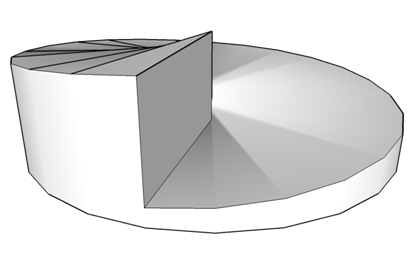
\includegraphics[width=1.37in]{illustrations/tomography/spp} % max width @300dpi
\caption{Sketch of a typical spiral phase plate.}
\label{tomography:fig:spp}
\end{marginfigure}
%
\begin{figure*}[tb]
\forceversofloat\centering
\includegraphics{graphs/tomography/halfvortex}
\caption{(a) Far-field diffraction pattern of a $Q = +3\half$ vortex beam; (b) experimental tomogram of this beam on slits separated by 25 \textmu m; (c) 75 \textmu m; (d) calculated tomogram of an ideal $Q=+3\half$ vortex beam on slits separated by 25 \textmu m; (e) 75 \textmu m.
Three intensity nodes are visible, but they are not arranged along a straight line.}
\label{fig5}
\end{figure*}

For a better understanding of the relation between the fractional part of the vortex charge and the presence and position of the fourth vortex in the tomogram, we calculated the tomograms of beams with various vortex charges between $+3$ and $+4$, shown in Fig.~\ref{tomography:fig:fractional}.
We see that as $Q$ increases, the fourth vortex, as seen in Fig.~\ref{fig5}, approaches the three existing vortices, and eventually joins them in a straight line at $Q=+4$.
The vortices are arranged in a straight line only when $Q$ is an integer.
This suggests that a non-integer vortex charge can be determined from the deviation of the vortices' arrangement from a straight line, the angle of which is determined mainly by the ratio of the distance between the slits to the spot size of the beam.
Our calculations indicate that any dependence on $Q$ is less than 1\textdegree\ and may be a numerical artifact.
%
%%%%% TWEAK %%%%%%%%%%%%%%%%%%%%%%%%%%%%%%%%%%%
\begin{figure*}[b]
\centering
\includegraphics{graphs/tomography/charge-evolution}
\caption{Calculated tomograms of vortex beams with $Q$ ranging from $+3$ to $+4$ on slits separated by 50 \textmu m.
(a) $Q=+3$; (b) $Q=+3\boxfrac{1}{4}$; (c) $Q=+3\half$; (d) $Q=+3\boxfrac{3}{4}$; (e) $Q=+4$.
The locations of the intensity zeroes are indicated with dots.
In (a) and (e), the size of the original vortex ring is superimposed on the tomogram.}
\label{tomography:fig:fractional}
\end{figure*}

\section{Summary}

\sectionstart{We have used the diffraction} of surface plasmon polaritons to analyze a vortex-carrying light beam slice by slice, in order to recover information about the beam's phase: specifically, its vortex charge.
Although the determination of non-integer vortex charges is not possible at a glance, we have shown through calculations that the magnitude of a non-integer vortex charge may be determined by measuring how much the arrangement of the vortices deviates from a straight line.

Phase retrieval normally requires some technique such as interferometry or a combination of near-field and far-field measurements. The current experiment's two slits can be considered to measure the surface plasmons' near field and far field. Therefore, the technique might be generalized to phase retrieval of arbitrary fields.
Also, the sample's small size and the small distances between the optics involved suggest that the experiment can be easily miniaturized.
Therefore, it has a potential application as a wavefront sensor.

\glsresetall

\part[Anomalous surface plasmon dispersion in aluminum]{Anomalous \\surface plasmon \\dispersion in \\aluminum}

% Tweaks: 4
\include{chapters/drudium}
\begin{appendices}
\include{chapters/drudium-appendix}
\end{appendices}
\glsresetall

% Bad vboxes: 1
\include{chapters/kretschmann}
\begin{appendices}
\include{chapters/kretschmann-appendix}
\end{appendices}
\glsresetall

\include{chapters/otto}
\begin{appendices}
\include{chapters/otto-appendix}
\end{appendices}
\glsresetall

\backmatter %%%%%%%%%%%%%%%%%%%%%%%%%%%%%%%%%%%%%%%%%%%%%
\bookmarksetup{startatroot} % Following chapters are not part of Part II

% Redefine 'bibintoc' heading so that it doesn't capitalize the running head
\defbibheading{bibintoc}[\bibname]{%
    \chapter*{#1}%
    \addcontentsline{toc}{chapter}{#1}%
    \markboth{#1}{#1}}
{\raggedright
\printbibliography[heading=bibintoc]}

\begin{otherlanguage}{dutch}

\nonumberchapter{Samenvatting}

\sectionstart{Een oppervlakteplasmon} is een lichtgolf die gebonden is aan een metaaloppervlak.
Er bestaan twee soorten van: de ene komt voor bij metalen deeltjes met sub-micron afmetingen, de andere bij metaaloppervlakken die tenminste op de schaal van de optische golflengte vlak zijn.
In dit proefschrift, \emph{``Tweedimensionale optica: diffractie en dispersie bij oppervlakteplasmonen,''} gaat het over het laatste type. Deze soort plant zich langs het twee-dimensionale metaaloppervlak voort, in tegenstelling tot `gewoon' licht dat door de driedimensionale ruimte reist.
De binding van oppervlakteplasmonen aan het metaaloppervlak maakt het mogelijk optische signalen te sturen door kanalen met extreem kleine afmetingen.

\section*{Deel 1: Verschijnselen bij dunne spleten in metaalfilms}

\sectionstart{Uit eerder werk,} o.a.\ dat van mijn voorganger Nikolay Kuzmin, was bekend dat onder bepaalde omstandigheden een zeer nauwe spleet of kras in een heel dunne metaallaag invallend licht met de juiste polarisatie om kan zetten in oppervlakteplasmonen, en omgekeerd.

In hoofdstuk~\ref{qwp:chapter} bekijken we bij een metaalfilm gemaakt van goud met een dikte van 0.0002 mm, hoeveel licht door spleten van verschillende breedte, varierend van 0.00005 tot 0.0005 mm, doorgelaten wordt, en hoe dit doorgelaten licht gepolariseerd is.
We gebruiken het aanslaan van oppervlakteplasmonen bij één polarisatie om de polarisatie van het doorgelaten licht te kunnen beheersen.
Het blijkt dat bij een bepaalde spleetbreedte en filmdikte de spleet lineair gepolariseerd licht kan omzetten in circulair gepolariseerd, en omgekeerd.
Wij hebben een simpel model ontwikkeld dat deze uitkomst ook op intuïtieve wijze verklaart.
Dit resultaat is een handige manier om op kleine schaal de functionaliteit van een zogenaamde kwart-lambdaplaat te realiseren.
In hoofdstuk~\ref{soc:chapter} gebruiken we dit verschijnsel nog eens, maar met cirkelvormige spleten, om een optische draaikolk te laten ontstaan uit circulair gepolariseerd licht, en daarmee optisch spinimpulsmoment om te zetten in optisch baanimpulsmoment.

Hoofdstuk~\ref{ch:tomography} beschrijft een proef met twee zeer nauwe spleten die in een heel dunne goudfilm parallel aan elkaar zijn gekerfd.
De ene spleet wordt beschenen met licht; dat wordt daar gedeeltelijk omgezet in oppervlakteplasmonen.
De oppervlakteplasmonen reizen naar de andere spleet waar ze weer omgezet worden in licht.
We meten de lichtverdeling, maar onderweg is deze door buiging van vorm veranderd ten opzichte van de verdeling bij het invallende licht.
Deze vormverandering gebruiken we om informatie over de fase (het golffront) van het invallende licht te achterhalen; de fase kan niet direct worden gemeten en wordt meestal gemeten met behulp van interferentie met een tweede lichtbundel.
Als toepassing van deze techniek meten we de fase van een bundel die een optische draaikolk bevat, maar uiteindelijk kan de techniek leiden tot een golffrontsensor met een veel hogere ruimtelijke resolutie dan de gangbare technieken, wat interessant zou kunnen zijn voor de astronomie en \smallcaps{UV}-lithografie.

\section*{Deel 2: Anomale dispersie van oppervlakteplasmonen}

\sectionstart{Dispersie is het verschijnsel} dat de snelheid waarmee licht zich door een materiaal voortplant afhangt van de golflengte van het licht (de kleur).
Bijvoorbeeld, een puls van rood licht en \'e\'en van blauw die op hetzelfde moment een blok glas worden ingestuurd, komen aan de andere kant op verschillende momenten aan.
Gewoonlijk komt het rode licht eerder aan dan het blauwe (deze situatie wordt `normale dispersie' genoemd), maar soms is het andersom: `anomale' dispersie.
Anomale dispersie heb je nodig om solitonen te laten ontstaan, lichtpulsen die een lange afstand kunnen afleggen zonder te vervormen.

Anomale dispersie komt vaak voor in de buurt van golflengtes die het materiaal absorbeert.
Het metaal aluminium heeft zo’n absorptie in het nabije infrarood.
In het tweede deel van dit werk proberen wij de vraag te beantwoorden of deze absorptie ook anomale dispersie van oppervlakteplasmonen aan een aluminiumoppervlak met zich meebrengt.
Dit onderzoeken wij met een methode, waarbij de oppervlakteplasmonen aangeslagen worden door licht aan te voeren vanuit een prisma.
Deze techniek kent twee varianten, genoemd naar de Duitse onderzoekers Kretschmann en Otto.
Van de Ottoconfiguratie wordt vaak gedacht dat deze alleen maar nadelen biedt vergeleken met de Kretschmannconfiguratie.
In hoofdstuk~\ref{ch:drudium} laten we zien dat dit een misverstand is.
Daarnaast introduceren we een analysemethode waarmee wij de resultaten van experimenten aan verliesgevende metalen met beide opstellingen zinvol kunnen interpreteren, wat niet mogelijk is met de gebruikelijke aanpak.

Hoofdstukken~\ref{ch:kretschmann} en~\ref{ch:otto} beschrijven de meetresultaten aan oppervlakteplasmonen met anomale dispersie.
In hoofdstuk~\ref{ch:kretschmann} tonen we inderdaad anomale dispersie aan bij oppervlakteplasmonen op een aluminiumoppervlak.
Vervolgens maken we de mate van anomale dispersie nog veel groter door het metaal tot vloeibare stikstoftemperatuur af te koelen, ongeveer $-200\unit{^\circ C}$, beschreven in hoofdstuk~\ref{ch:otto}.
Dit is echter een afweging tussen meer anomale dispersie en meer verlies, omdat de oppervlakteplasmonen sneller uitdoven op het gekoelde metaal.

\end{otherlanguage}

\nonumberchapter{Curriculum Vit\ae}

\section*{Philip Francis Chimento \smallcaps{III}}

\begin{fullwidth}
\begin{tabular}{lp{10cm}}
1981       & Born in Raleigh, North Carolina, United States \smallskip \\
1993--1994 &
	{\raggedright Secondary education, Sherwood Githens Middle School, Durham, \\
	North Carolina, United States} \smallskip \\
1994--1999 & Secondary education, \foreignlanguage{dutch}{Het Stedelijk Lyceum}, Enschede, Netherlands \smallskip \\
1999--2008 &
	{\raggedright Bachelor's and Master's degree in applied physics \\
	Twente University, Enschede, Netherlands \\
	\emph{Freshman year completed cum laude}}
	\smallskip \\
2009--2013 &
	{\raggedright PhD research \\
	Leiden Institute of Physics, Leiden University, Leiden, Netherlands}
	\smallskip \\
2013--     & Software engineer, Endless Mobile
\end{tabular}
\end{fullwidth}

\nonumberchapter{List of Publications}
{\raggedright
\begin{itemize}
\item Chimento, P.~F., Jurna, M., Bouwmans, H.~S.~P., Garbacik, E.~T., Hartsuiker, L., Otto, C., Herek, J.~L., \& Offerhaus, H.~L.\ (2009). High-resolution narrowband \smallcaps{CARS} spectroscopy in the spectral fingerprint region. \emph{Journal of Raman Spectroscopy, 40,} 1229--1233.
\item Chimento, P.~F., 't~Hooft, G.~W., \& Eliel, E.~R.\ (2010). Plasmonic optical vortex analyzer. In J. Pozo, M. Mortensen, P. Urbach, X. Leijtens, \& M. Yousefi (Eds.), \emph{Proceedings of the 2010 annual symposium of the \smallcaps{IEEE} Photonics Benelux Chapter,} November 19, 2010 (pp. 17--20). 2010 Annual Symposium of the \smallcaps{IEEE} Photonics Benelux Chapter. Delft, Netherlands: Uitgeverij \smallcaps{TNO}.
\item Chimento, P.~F., 't~Hooft, G.~W., \& Eliel, E.~R.\ (2010). Plasmonic tomography of optical vortices. \emph{Optics Letters, 35,} 3775--3777.
\item Chimento, P.~F., Kuzmin, N.~V., Bosman, J., Alkemade, P.~F.~A., 't~Hooft, G.~W., \& Eliel, E.~R.\ (2011). A subwavelength slit as a quarter-wave retarder. \emph{Optics Express, 19,} 24219--24227.
\item Chimento, P.~F., Alkemade, P.~F.~A., 't~Hooft, G.~W., \& Eliel, E.~R.\ (2012). Optical angular momentum conversion in a nanoslit. \emph{Optics Letters, 37,} 4946--4948.
\item Chimento, P.~F., 't~Hooft, G.~W., \& Eliel, E.~R.\ (2013). When the dip doesn't tell the whole story: interpreting the surface plasmon resonance in lossy metals. Submitted to \emph{Optics Express}.
\item Chimento, P.~F., 't Hooft, G.~W., \& Eliel, E.~R. Anomalous dispersion of surface plasmons. In preparation.
\item Chimento, P.~F., 't Hooft, G.~W., \& Eliel, E.~R. Enhancing the anomalous surface plasmon dispersion in aluminum. In preparation.
\end{itemize}
}

\nonumberchapter{Acknowledgements}

\sectionstart{I would most like to thank} the students that I had the pleasure of mentoring: Carolina Rend\'on Barraza, Johan Bosman, Mark Bogers, David Kok, and Tobias de Jong.
They all contributed in important ways, even though the project that Carolina, David, and Tobias worked on did not make it into the publishable stage because of time constraints.

One is not allowed any more to thank one's coworkers indiscriminately, but some people deserve a mention for their contributions beyond those of the co-authors on my papers.
Wolfgang L\"offler's expertise is woven all throughout this book; he was always ready to bounce ideas off and share lab tips.
Michiel de Dood took a special interest in the aluminum project (chapters~\ref{ch:kretschmann} and~\ref{ch:otto}) and our discussions were invaluable in understanding the solid-state physics involved.
Daan Boltje put time into preparing the Kretschmann prisms used in chapter~\ref{ch:kretschmann}.

The work described in chapter~\ref{ch:otto} involved cryostats and liquid nitrogen, something I had had little experience with when I started.
Jelmer Renema helped to close this experience gap, and assisted with the \smallcaps{COMSOL} heat flow simulations.
Mirthe Bergman, Arjen Geluk, and others in the Fine Mechanics Department worked on the cryostat that I used and made sure it was simple, easy, and leak-free.

Philippe Lalanne, professor at the Institut d'Optique, \smallcaps{CNRS}, was willing to share the Gaussian quadrature code from their paper\cite{Lalanne2006} which I adapted for chapter~\ref{qwp:chapter}.
Speaking of sharing computer code, I relied heavily on open source software almost from the start of this research.
NumPy and SciPy\cite{Jones2001} did all the number crunching.
I made all the graphs in this book with Matplotlib\cite{Hunter2007} and the diagrams with Inkscape.
I used DataThief \smallcaps{III}\cite{Tummers2006} to digitize printed specs of anti-reflection coatings.

% Bring number of pages to a multiple of 4
\newpage
\thispagestyle{empty}
\mbox{}
\newpage
\thispagestyle{empty}
\mbox{}
\newpage
\thispagestyle{empty}
\mbox{}


\end{document}
